\documentclass
[
	paper = a4,
    pagesize,
	12 pt,
	oneside,                       % Chose ›oneside‹ for digital version, ›twoside‹ for printed version.
    open = right,
	DIV = calc,
	BCOR = 0 mm,                   % Binding correction. Only necessary for printed version. Depends on actual binding.
	bibtotoc
]
{scrbook}

% Do not change the following commands.
\newcommand*{\printTitle}{}
\newcommand*{\printAuthor}{}
\newcommand*{\printDateOfBirth}{}
\newcommand*{\printPlaceOfBirth}{}
\newcommand*{\printSubject}{}
\newcommand*{\myTitle}[1]{\renewcommand*{\printTitle}{#1}}
\newcommand*{\myName}[1]{\renewcommand*{\printAuthor}{#1}}
\newcommand*{\myDateOfBirth}[1]{\renewcommand*{\printDateOfBirth}{#1}}
\newcommand*{\myPlaceOfBirth}[1]{\renewcommand*{\printPlaceOfBirth}{#1}}
\newcommand*{\mySubject}[1]{\renewcommand*{\printSubject}{#1}}

\myTitle{High-level Visualization of Graph Algorithms}  % Change!
\myName{Julius Milian Severin}  % Change!
\myDateOfBirth{March~12, 1995}  % Change!
\myPlaceOfBirth{Berlin, Germany}  % Change!
\mySubject{{Graph Algorithms}{Visualization}}  % Change!

\usepackage[utf8]{inputenc}
\usepackage[T1]{fontenc}
\usepackage[english]{babel}

\usepackage{graphicx}

\graphicspath{{Images/}}

\usepackage{pgf}

\usepackage							% Microtypography tuning.
[
	protrusion = true,
	expansion = false,
	tracking = true,
	kerning = true,
	spacing = false,
	babel = true
]
{microtype}							% http://ctan.mirrorcatalogs.com/macros/latex/contrib/microtype/microtype.pdf

\SetTracking[unit = space]{font = */*/*/sc/*}{25}   % Adjust kerning for small caps.

\SetExtraKerning[unit = space]		% Adjusted kerning for certain characters.
{
	font = */*/*/*/*
}
{
	: = {100, },
	; = {100, },
	? = {150, 150},
	! = {150, 150},
	: = {250, },
	; = {150, },
	? = {250, 250},
	! = {250, 250},
	» = { , -200},
	« = {-200, },
	› = { , -200},
	‹ = {-200, },
	– = {200, 250},
	— = {200, 250},
	@ = {200, 200}
}

\usepackage{booktabs}
\usepackage{breakurl}
\usepackage{emptypage}

\usepackage[bottom]{footmisc}
\usepackage{remreset}

\makeatletter
    \@removefromreset{footnote}{chapter}
\makeatother

\renewcommand*{\footnoterule}{\rule{0 pt}{0 pt}}
\deffootnote[1.2 em]{1.2 em}{0 em}{\makebox[1.4 em][l]{\textbf{\thefootnotemark}}}

\usepackage{xparse}

\DeclareDocumentCommand{\myfootnote}{o o o m}
{%
    \IfNoValueTF{#1}%
    {%
        \footnote{#4}%
    }%
    {%
        \IfNoValueTF{#2}%
        {%
            \kern #1 em\footnote{#4}%
        }%
        {%
            \IfNoValueTF{#3}%
            {%
                \kern #1 em\footnote{#4}\kern #2 em%
            }%
            {%
                \kern #1 em\footnote[#3]{#4}\kern #2 em%
            }%
        }%
    }%
}

\usepackage{titlesec}

\titleformat{\chapter}
    {\normalfont\rmfamily\huge\bfseries}
    {\thechapter}{1 em}{}

\titleformat{\section}
    {\normalfont\rmfamily\Large\bfseries}
    {\thesection}{1 em}{}

\titleformat{\subsection}
    {\normalfont\rmfamily\large\bfseries}
    {\thesubsection}{1 em}{}

\titleformat{\subsubsection}
    {\normalfont\rmfamily\normalsize\bfseries}
    {\subsubsectionname}{1 em}{}


\pagestyle{headings}

\usepackage{amsmath}
\usepackage{amssymb}
\usepackage{amsfonts}
%\usepackage{upgreek}               % Use if you want to use upright lowercase and italic upercase greek letters.
%\usepackage{dsfont}                % Use if you want to use special symbols.

%\usepackage[printonlyused]{acronym} % Use if you want to have acronyms. http://mirror.hmc.edu/ctan/macros/latex/contrib/acronym/acronym.pdf

%\usepackage{pifont}				% Special symbols.
%\usepackage{fourier-orns}			% More special symbols.
\usepackage{lettrine}

\usepackage{enumitem}
\usepackage
[
	format = plain,
	textfont = {sf, footnotesize},
	labelfont = {sf, bf}
]
{caption}[2008/08/24]
\usepackage{subcaption}				% For using sub-figures.

\usepackage
[
    algo2e,
    ruled,
    vlined,
    linesnumbered,
    algochapter
]
{algorithm2e}

\SetAlCapFnt{\sffamily\footnotesize}
\SetAlCapNameFnt{\sffamily\footnotesize}

\usepackage[numbers]{natbib}

\makeatletter
    \def\NAT@spacechar{~}% NEW
\makeatother

\definecolor{darkblue}{rgb}{0, 0, 0.5}

\usepackage
[
	bookmarks = true,
	bookmarksopen = false,
	bookmarksnumbered = true,
	pdfstartpage = 1,
	pdftitle = {{\printTitle}},
	pdfauthor = {{\printAuthor}},
	pdfsubject = {{\printSubject}},
	backref = page,
	breaklinks = true,
	colorlinks = true,
	linkcolor = darkblue,
	anchorcolor = darkblue,
	citecolor = darkblue,
	filecolor = darkblue,
	menucolor = darkblue,
	pagecolor = darkblue,
	urlcolor = darkblue
]

\usepackage{hyperref}


\renewcommand*{\backref}[1]{}
\renewcommand*{\backrefalt}[4]
{
    \ifcase #1
        Not cited.
    \or
        \footnotesize (Cited on page #2.)
    \else
        \footnotesize (Cited on pages #2.)
    \fi
}

\usepackage{cleveref}

\begin{document}




\begin{document}


\frontmatter
% Title Page
\thispagestyle{empty}
\begin{center}
    {\Huge \textbf{\printTitle}}\\[7 ex]
    {\Large\textsc{Bachelor Thesis}}\\[4 ex]    
    {\large
        to attain the scientific degree\\[4 ex]
        \textbf{Bachelor of Science}
    }
    \vfill
    \includegraphics[width = 8 cm]{HPI_logo.pdf}\\[8 ex]
    \begin{tabular}{l}
        handed in by \textbf{\printAuthor}\\[1.1 ex]
        born \printDateOfBirth, in \printPlaceOfBirth\\[3 ex]
        \textbf{Advisor:} Prof.~Dr.~Tobias Friedrich\\[9 ex]
    \end{tabular}
    
    Potsdam, \today
\end{center}

% Abstract
\chapter*{}
\addcontentsline{toc}{chapter}{Abstract}
\thispagestyle{empty}

\begin{center}
    \large \textbf{Abstract}
\end{center}

Developing an algorithm is an iterative process.
Therefore an understanding of the different approches is important.
Furthermore, as the algorithm becomes more complex, it may come to different results than expected, when running on real data.

This thesis deals with those issues on the example of shortest path algorithm on tiled map data.
Therefore, multiple ways of visualizing a shortest path algorithm with respect of this specific class of algorithms are introduced.
Using those methods we were able to archieve a better understanding of the algorithms and built a powerful basis for discussions.
In addition we enabled the researchers to find the missbehaviour more easily.

\chapter*{}
\addcontentsline{toc}{chapter}{Zusammenfassung}
\thispagestyle{empty}

\begin{center}
    \large \textbf{Zusammenfassung}
\end{center}

Das Entwickeln eines Algorithmusses ist ein iterativer Prozess.
Daher ist es wichitg, dass alle Beteiligten, die verschiedenen Ansätze verstehen.
Ausserdem kann es mit wachsender Komplexität des Algoithmus dazu kommen, dass sich der Algorithmus auf echten Daten anders verhalten als gedacht.
Das finden der Ursache kann ein äußerst komplexes Verfahren sein.

In der folgenden Arbeit erklären wir, wie wir die Entwicklung eines Algorithmus zum finden kürzester Wege durch eine Visualisierung untersützt haben.
Dabei gehen wir auf die Probleme ein, die wir wärend der Entwicklung der Visualisierung lösen mussten.


% Table of Contents
\renewcommand*{\listfigurename}{\normalfont\rmfamily\Large\bfseries List of Figures}
\renewcommand*{\listtablename}{\normalfont\rmfamily\Large\bfseries List of Tables}
\pdfbookmark{\contentsname}{toc}
\microtypesetup{protrusion = false}
    \tableofcontents
    \begingroup
    \let\clearpage\relax
    \listoffigures                  % Comment out if necessary.
    \listoftables                   % Comment out if necessary.
    \endgroup
\microtypesetup{protrusion = true}


\mainmatter
\chapter{Introduction} \label{introduction}
Graphs are a common structure in computer science.
Therefore developing more efficient graph algorithms plays a big role in algorithm engineering.
During the process of development knowing how the algorithm behaves is really important.
Firstly developing an algorithm is an iterative process it is fundamental to communicate about the different approaches and therefore create an understanding of them in the whole team.
Furthermore, the developed algorithms can become quite complex and therefore the idea of how the algorithms should behave and the way they actually behave on real graph data can diverge quite a lot.
\par
As the eyes are a fast way to access information a good way to achieve this understanding is to visualize the progress of the algorithm.
Though there are many tools for visualizing graphs, there is still a lack of algorithm visualization tools.
Therefore writing an own visualization that fits one's needs might be necessary.
In the following, we will describe the process of developing a sensemaking visualization the example of a shortest path algorithm. The algorithm was developed on a geographical tiled road network with the special requirement to reduce the amount of tile-accesses during the algorithm.


\chapter{Preliminaries} \label{questions}

In this chapter, we will lay the foundation on which we are going to build the visualization in \cref{main}.
\newline Thereby in \cref{specification} we are going to look at the basis of the algorithm that is going to be visualized, the data the algorithm is running on and finally combine both and therefore continue on how the given data influences the algorithm.
In the following sections, we are going to take a look at questions that need to be answered for developing the visualization.
Those will then be answered in the corresponding sections in \cref{main}

\section{Problem Specification} \label{specification}

% Routing
The algorithm that is going to be displayed in out visualization is a graph algorithm, or more precisely a shortest path algorithm.
A shortest path algorithm, in general, has the goal to find a path from a start node to a target node in a graph.
A graph consists of multiple node and edges.
Thereby an edge connects exactly two nodes in either one direction, in a directed graph, or both directions, in an undirected graph.
Depending on the graph nodes and/or edges can be so-called weighted, which describes the costs that occur when a route passes the element.
The shortest path algorithm has to find a path with the smallest possible summed costs.

% Basic algorithm
\par The groundwork of the algorithm was the so-called Dijkstra algorithm and its improvement the A*-algorithm.
The Dijkstra algorithm starts at the start node wherefrom it observes its neighbors, the nodes that are connected to the start node by an edge.
At any point, the algorithm can observe any neighbor of the already explored nodes.
It decides which node should be explored next, depending on the overall path costs from the start node.
The algorithm is done as soon as it observes the target node.
This leads to a more or less circular spreading around the start node.
The A*-algorithm adopts a similar strategy with the difference that it uses some heuristic which leads to a more target-oriented spreading and therefore less observed nodes which means a faster algorithm.

% Data
\par The graph the algorithm is running on was derived from a road network.
Therefore every node represents a crossing point and every edge stands for a street or even a ferry route.
For our graph this means that the edges are directed and have a certain weight, which can be calculated using the speed of the edge and its length.
In addition, every node has given a pair of coordinates, which refers to a certain position on the Earth.
The special thing about the graph is a geographical grid that divides the graph into tiles.
Therefore every node belongs to exactly one tile which is accessed whenever one of the related tiles is observed.
Those tiles have been introduced by the Navigation Data Standart (NDS) which requires that every tile is encrypted and compressed.

% impact
\par The NDS impacts the algorithm in so far as accessing tiles becomes the major effort, as decrypting and decompressing is costly and therefore time-consuming.
Hence the algorithm should access as little tiles as possible.
As the algorithm is developed for portable devices, the algorithm has access to the so-called cache, a fast storage with limited size.
Since tiles can be stored in the cache, accessing a tile is only costly whenever it is not in the cache.
Due to the limited size of the cache, loading a tile requires removing another, as soon as the cache is full.


% Before building a visualization we need to develop an understanding for the graph and the purpose the algorithm shall be developed for.
% The algorithm is going to be a shortest pathalgorithm, that shall find the shortest way from one node to an other. Thereby a node represents a crossing point of two roads which are represented by edges.
% Therefore every node has given coordinates which stand for the position of the node on the earth.
% As an edge represents a street it has given a length and a speed.
% Every edge connects exactly two nodes.
% Each node belongs to exactly one tile.
% The tiles divide the graph according to a geographical grid and have been introduced by the Navigation Data Standart(NDS).
% Due to the NDS the tiles are encrypted and compressed and therefore the aim of the algorithm is to load tiles as rare as possible.
% A tile needs to be loaded whenever a node should be accessed which is not loaded.
% When a tile is loaded it is stored in the cache, a fast storage
% of limited size. As the size of the cache is limited, a tile needs to be removed when the cache is full and a new tile shall be loaded. Therefore this tile would need to be loaded again when it is accessed another time.
% During the development of the algorithm the assumption was made, that the cache fits a fixed amount of tiles.


\section{Displaying the Graph} \label{graph}

For developing a visualization of a graph algorithm it is probably useful to think about the basics and therefore about how to display the graph itself first.
For displaying the graph we will have to think about how we are going to arrange the nodes on the screen.
As we already have some positioning of the notes, even though it is based on a three-dimensional body, this might be a good starting point.
\\After having figured this out, we need to discuss the way we are going to represent nodes and edges.
Therefore we will evaluate common methods used by e.g. teaching.


\section{Displaying the Algorithm}

In this section, we will take a look on how to transform the static representation of the graph to visualization of an algorithm.
The challenge here is to transform the graph to a sequence of multiple states of the algorithm.
Furthermore, we are going to examine how to include all information in the visualization, necessary to support the researcher in understanding and developing the algorithm.


% Even though visualizing graphs on a high level is a common thing and impressive graphs is an even used for marketing reasons (e.g. Facebook), visualizing algorithms itself is mostly seen in doctrine on a small scale.


\subsection{Basics}

For building the visualization we need some basis, which we will then customize till it fits out needs.
This basis is going to be formed here.
We will have to decide how the visualization starts and how the process of the evolving graph can be shown.
We need to think about how to place the displayed on the screen and whether and, if so, how we are going to label the start and the target of the algorithm.

% Since the visualization of graph algorithms is not such common, there are multiple basic questions that need to be answered.
% Which segment should be shown in the beginning? How to visualize the progressing algorithm?
% And which basic features should be included for increasing the accessibility of the information displayed.
% \todo{how to display start and end}
% \todo{Maybe put this to Micellaneous}


\subsection{Displaying the Tiles}

As we are going to have a basic idea on how to visualize a graph.
Hence we can now start thinking about how to modify the visualization for fitting more the introduced graph and algorithms presented in \cref{specification}.
Therefore we will take a look at possibilities of representing the tiles in the visualization.

% The in \cref{specification} we already introduced the tiles that play a major role in the algorithms developed.
% Therefore we need to find a way to make the tiles visible for the user.


\subsection{Visualizing the Cache}

Now that we found a way to represent the tiles, we can finally find a way how to make the cache visible.
Firstly we want to know at every point which blocks are in the cache.
Furthermore, the information how often is in fact the most important information to display, as the goal of improving the algorithm is, to reduce the amount of overall tile loads as much as possible.
Hence it would be highly desirable to recognize how well an algorithm performs at one glace.
Moreover, it should be possible to analyze a specific algorithm and to determine in which regions perform better or worse.

% In the algorithms that should be developed the cache plays a role as well.
% Tiles only need to be loaded when they are not in the cache yet.
% So the relevant information is not how often a tile is accessed but how often a tile is accessed when it was not in the cache before.
% Hence we need to find a way to display that information as well.


\section{Compare algorithms}

As during the algorithm research multiple approaches are developed, there is the need to compare those approaches.
In this section, we will tackle this challenge and think about a possibility to compare two algorithms.

% After having answered all those questions introduced in the previous chapters we might also want to compare different algorithms. Is there maybe a way that includes more than just starting the visualization with two different algorithms and put them next to each other?


\section{Miscellaneous}

Now that we are able to visualize algorithms on a higher-level, we will develop even add some information to the visualization, or increases the accessibility of the information.


% In the end we will discuss some additional fancy features to give the visualization the last fancy touch.



\chapter{Buillding the Visualization} \label{main}

In this chapter we will discuss the questions introduced in \cref{questions}.


\section{Displaying the Graph} \label{graph}

In \cref{graph} we already introduced some issues we need to think about which will happen in this section.
In this process we will start taking a closer look on how to arrange the nodes on the sceen.
In \cref{specification} we learned that every node given coordinates according to their position on the earth.
As there are already many projections that map the coordinates of the three-dimensional earth to a sepcific position on a two-dimensional representation.

A very intuitive way of projecting coordinates is the Equirectangular projection.
The Equirectangular projection uses the coordinates as coordinates of a two-dimensional, linear scaled coordinate system. Therefore the longitude is used as x-value and the latitude as y-value.

The probably most common projection is the Mercator projection.
The Mercator projection was originally developed for nautical cartography in 16th century.
As the distance between the medians get smaller the closer we come to the poles, the map becomes more and more distorted the closer it comes to the poles.
Therefore the Mercator projection increases the distance between the latitudes.
This leads on the one side to a nondistorted map that hence can be used for nautical navigation, but on the other side this leads to the effect that countries on or close to the equator appear much smaller than more distant ones.

%This section we will take a closer look at the problematics introduced in \cref{graph} starting by the problem of aranging the nodes.
% As every node has given unique coordinates we will use those to arrange them on the screen.
% Therefore there are already many projections that calculate the position on the screen for given coordinates.
% The porbably most intuitive way of projecting coordinates is to just see the longitude and the latitude as coordinates on a two-dimensional graph.
% This projection is called Equirectangular projection.
% \par
% An other common projection is the Mercator Porjection.
% In Mercator projection the longitudes are all equally spaced but the latitudes move away from each other the bigger the distance to the equator becomes.

\todo{center the first image}

\begin{figure}[H]
	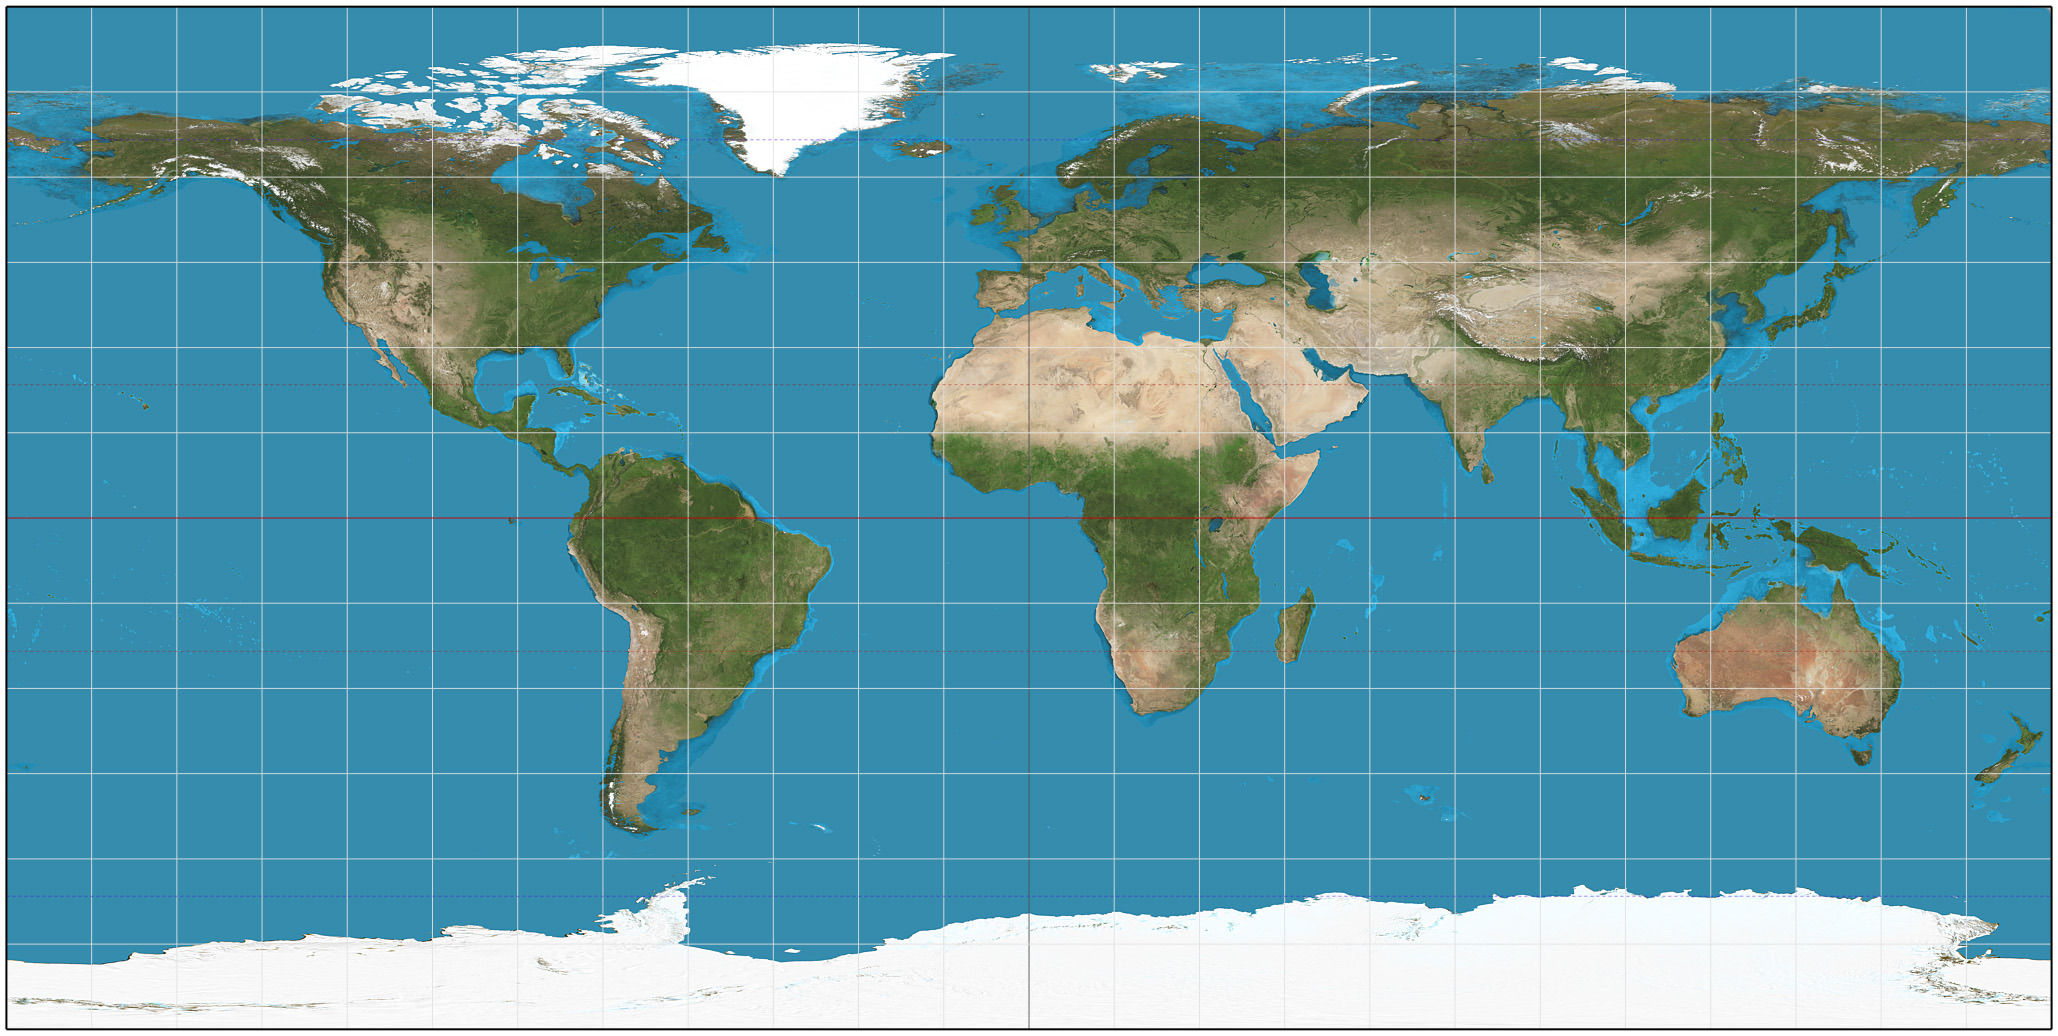
\includegraphics[width=.5\textwidth]{Images/Equirectangular_projection_SW.jpg}
	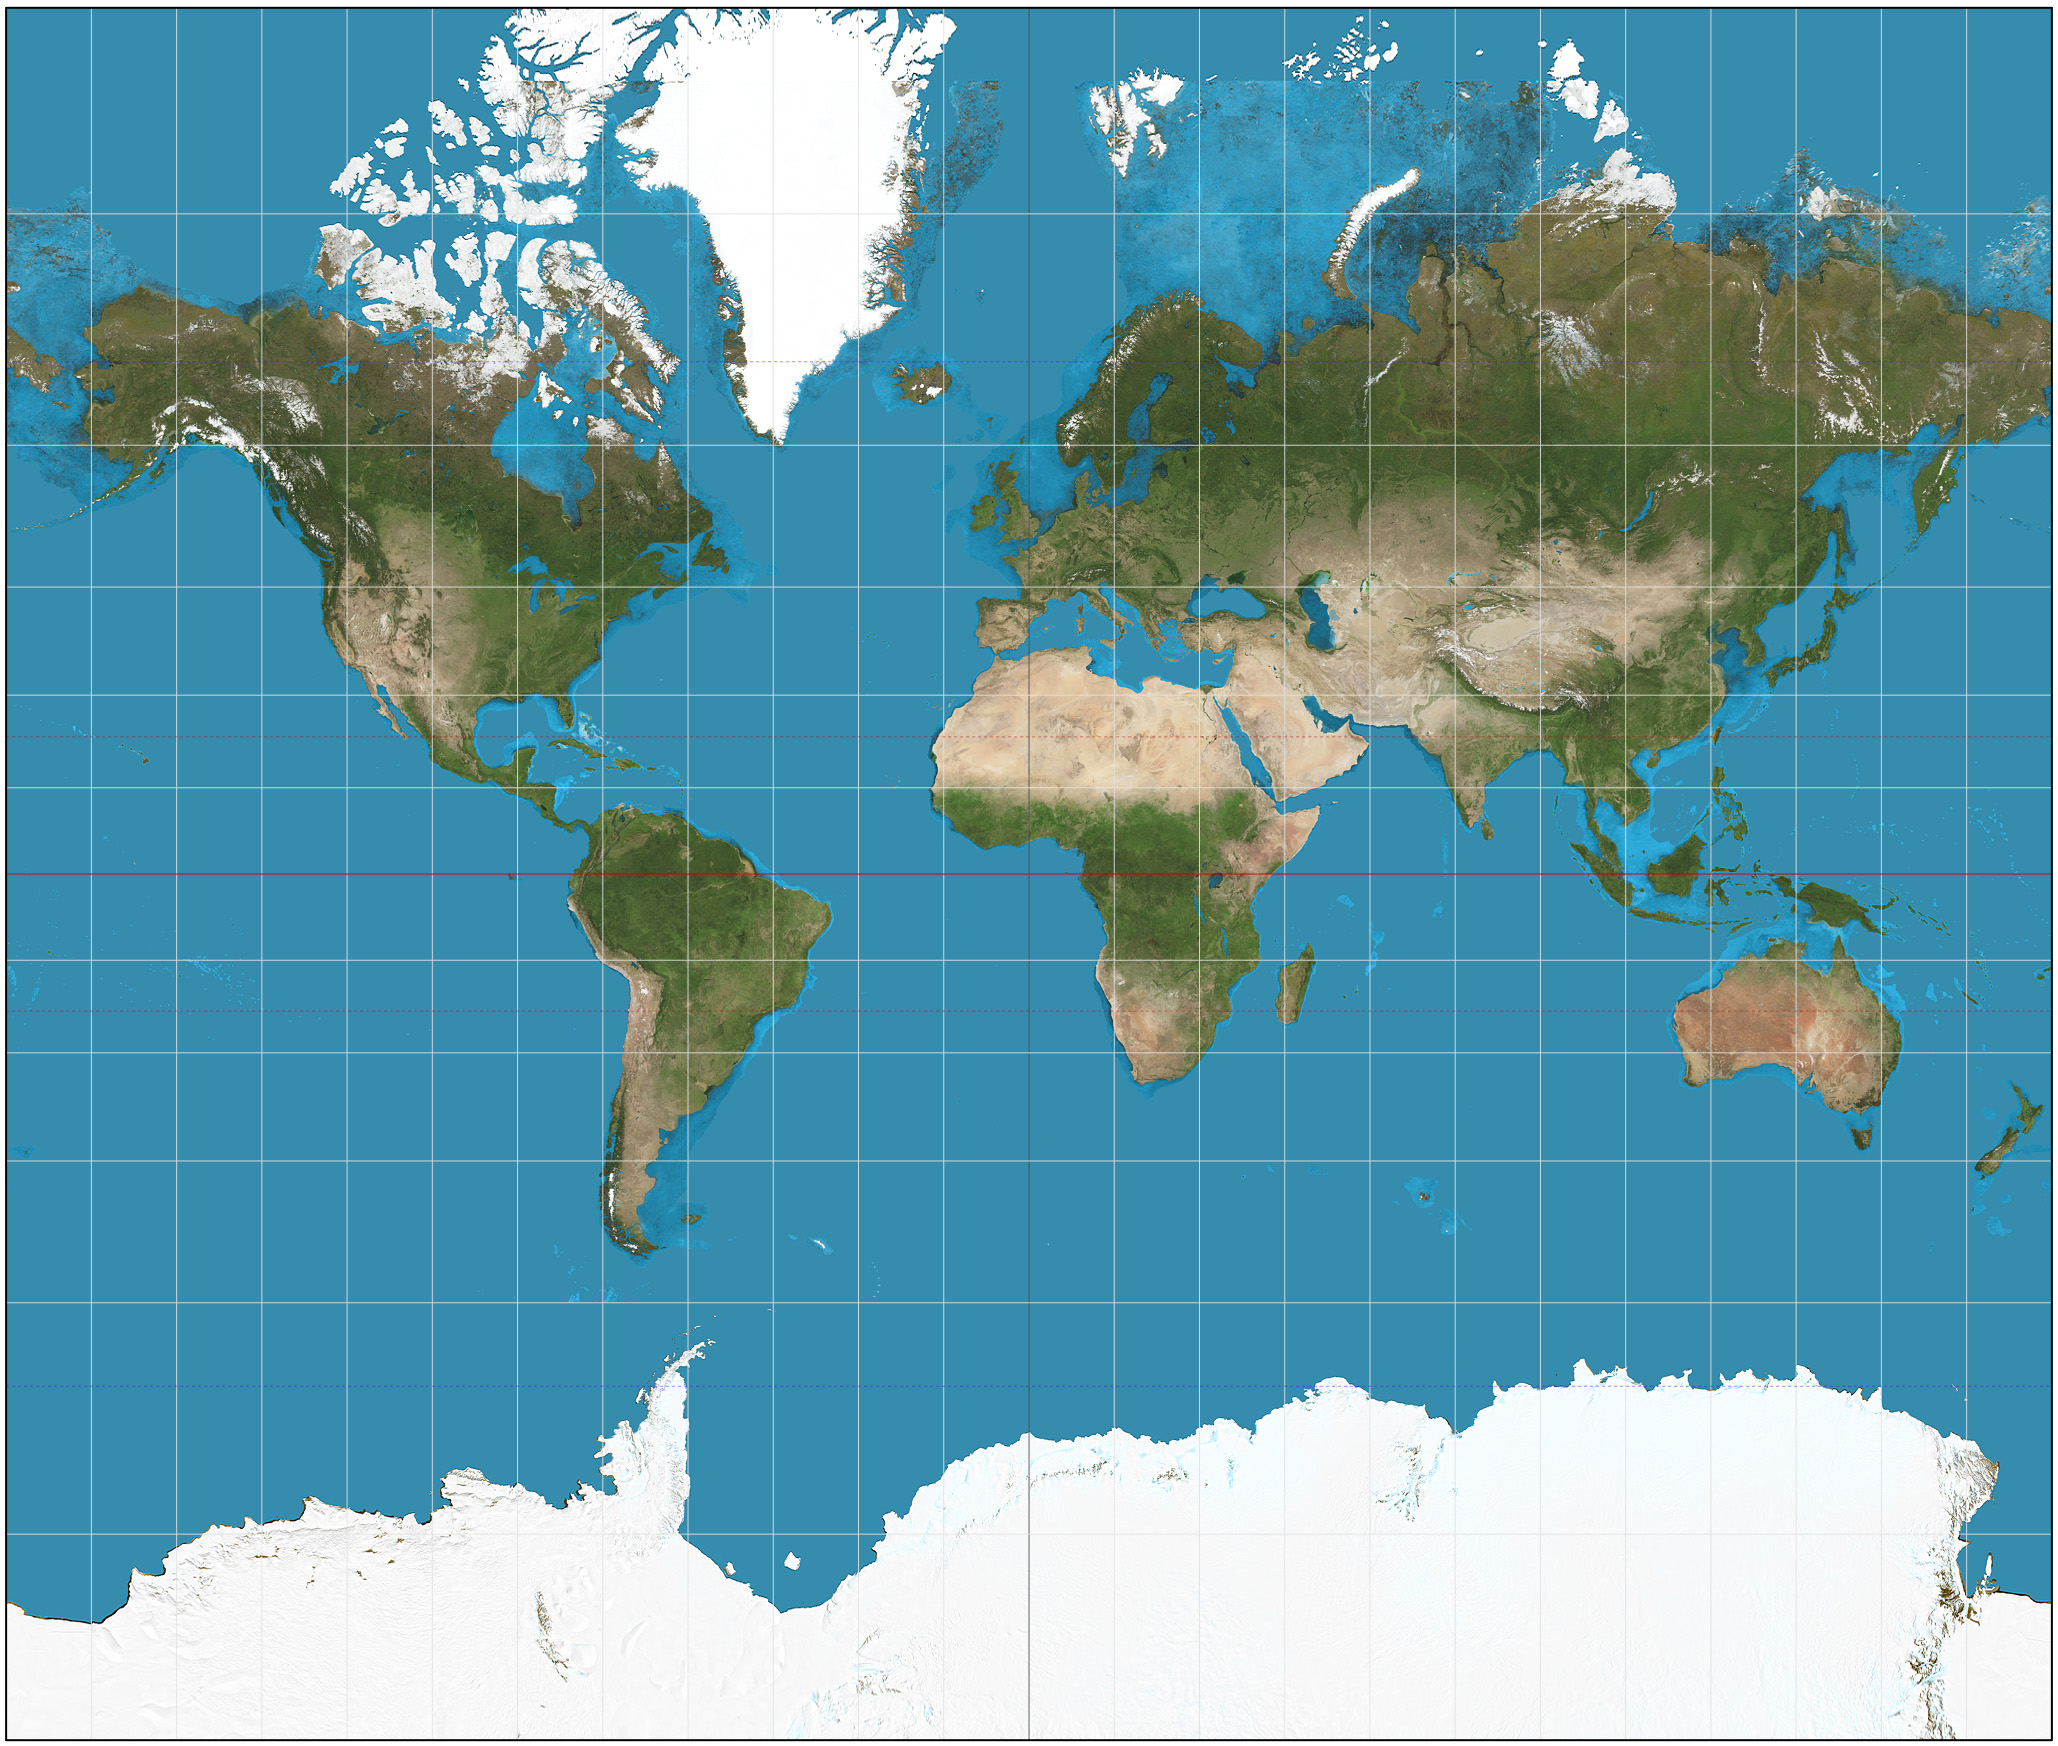
\includegraphics[width=.5\textwidth]{Images/Mercator_projection_SW.jpg}
\caption[]{Equirectangular projection(left) vs. Mercator projection(right)}
\label{fig:projections}
\end{figure}

As we see in \cref{fig:projections} the difference between both projections is not that big.
In the more northern and southern regions regions as Northern Canada the difference becomes bigger and the Mercator projection might be the better choise.
As the graphs we are going to run the algorithm an therefore the visualization on are mostly from central europe or northern america, they are not far enough as that the mercator projection would add enough value as that is would be worth the added complexity in calculation.
Therefore we are going to continue building the visualization using the  Equirectangular projection.

%
% As we see in \cref{fig:projections} the difference of both projections is not that serious.
% The only in extreme northern/southern areas the differencee is clearly visible.
% As mercator is used in most notable map representations as for example Google Maps and is often used for navigation it might be desirable to use mercator.
% Though most graphs we will be wokring on do not lie in those extreme areas an thus the added value is not worth the added complexity in calculation.
% Therefore we will use the Equirectangular projection for our visualization.


\paragraph{Edges}
As we already decided how to arrange the nodes on the graph.
Therefore the most straight forward way would be to display edges by connecting the nodes with a straight line.
This would also correspnd to most graph visualizations.
As the pure distance between the nodes does not necessarily match the length of the edge we could also think about a way to display it more correctly.
An idea would be to bend the edges depending on the factor between the air distance between two edges and the length of the edge.
Scince the air distance  and the length of the connecting edge do not differ greatly in most cases we decided to to stick with the straight lines, as the bounded lines would mean a much higher complexity in calculation and might result in a less understandable graph.

% It is common to display edges as straight lines.
% We could try to display the length or even the costs of the edge by bending them depending on the height of the value.
% As the air distance between two nodes and the length of the connecting edge does not derrive that much in general we will display edges by simple straight lines in the visualization.


\paragraph{Nodes}
In most common visoalizations of graphs, as they are mainly used in teaching, nodes are represented as circles.
As those visualizations are mostly used for smaller graph we should reconsider this representation of nodes.
Scince we know that every edge connects exactly two nodes, we can clearly identify a node by the ending of an edge as long as the node is connected to the graph.
Therefore we should consider to not add any additional representation of those nodes to the visualization as they do not any value to it and only make the visualitzation more crowded.
But what happens to the remaining nodes, that are not connected to any other?
As the only way for those nodes to play a role during our algorithm would be to be the start or the target node, we can just not visualize them for the sake of better clarity.

% In most visualizations of graph algorithms, that are mainly used for teaching, nodes are represented by circles.
% Though those visualizations perform only on small graphs and are went threw step by step.
% As we are going to display much bigger graphs we have to take a look at representation of nodes as well.
% In our graphs every node is connected to at least one edge. If not, the only way for the node to be accessed during our algorithms would be to be the start or the target node of the algorithm.
% As every node belongs to at least one edge a vizual representation of the node itself is redundant, as it is already represented by at least one end of an edge.



\section{Displaying the Algorithm}

In this section we are going to take a look on how to transform the visualization the graph itself, as discussed in \cref{graph} in a visualization of an algorithm.

% In this section we are going to the core of the visualization. Except of visualizing one state of the graph, we now want to create a way to see graph changes during the algorithm.


\subsection{Basics}

The difference between the visualization of a graph and an algorithm of a graph is that the visualization of an algorithm is a process which means that we want to be able to understand what is happening during the algorithm at any step.

Therefore a first visualization would starts with an empty space to which edges are added in the order they has been processed during the algorithm.

\begin{figure}[H]
	\includegraphics[width=.5\textwidth]{Images/placeholder.png}
	\includegraphics[width=.5\textwidth]{Images/placeholder.png}
\caption[]{Two consecutive steps in the visualization}
\label{fig:projections}
\end{figure}

In \cref{fig:projections} we can see quite well that this way to visualize the algorithm is a good beginning an helps to understand how the search front evolves quite well.
As the displayed graph grows in during the algorithm we have to think about which part of the graph we want to display during the visualization and how we want to make sure that every step of the algorithm can be observed as good as possible.
Thereby we have to respect that we have to chose the section big enough to see every action happening during the algorithm, but small enough to have as little space as possible unused when the search front is fully evolved.
Therefore we could on the one hand take the start and the end node as core which will be accessed at minimum.
As this would not be a big enough section of the graph as algorithms also have to consider routes that do not move straight in the direction of the target.
Hence we would try to estimate the most outer points of the search front and add a margin depending on this estimation.
Another way of setting the view on the algoithm is to examine all edges processed before we even start visualizint the algorithm.
Thereby we could calulate the exact borders of the search front.

\begin{figure}[H]
	\includegraphics[width=.5\textwidth]{Images/placeholder.png}
	\includegraphics[width=.5\textwidth]{Images/placeholder.png}
\caption[]{Estimation method with quite a good estimation(left) vs. Preprocessing method(right)}
\label{fig:sections}
\end{figure}

As the second method finds the correct extend of the graph we will display, we prefer this method over the other though the precision comes with higher costs which will lead to a higher initial loading time of the visualization.
As we want to build a visualization that is as understandable as possible the knowledge about the extend of the search front is worth the additional inital loading time to us.

Now that we found the section we want to display there would still be a possibility to minimize the empty space on our screen.
Currently we are using the same scale on the x-axis and the y-axis.
Therefore there could be a bigger empty space on one axis, as the scale would be set in regard of the broader direction of the search front.
Therefore we could also just change the scale of the slimmer direction of the graph and thus spread the graph over the whole screen.

\begin{figure}[H]
	\includegraphics[width=.5\textwidth]{Images/placeholder.png}
	\includegraphics[width=.5\textwidth]{Images/placeholder.png}
\caption[]{Same scaled axes(left) vs. Spreaded axes(right)}
\label{fig:spreaded_axis}
\end{figure}

As we see in \cref{fig:spreaded_axis} this reduces the unused space to a minimum.
Though we would loose a lot of unerstandibility, as the length of a line on the screen would indicate the length of the real edge even less.
Therefore uniform scaled axes are the better choice for a graph visualization.


\subsection{Displaying the Tiles} \label{tiles}

In \cref{specification} we described that the graph is splitted into tiles, which due to their encryption and compression should be loaded as rarely as possible.
Therefore the tiles are the major cost factor during the algorithm and thus should be respect in the visualization.
A first idea for doing this is to just display all edges of a tile as soon as a node of this tile has been accessed the first time.

\begin{figure}[H]
	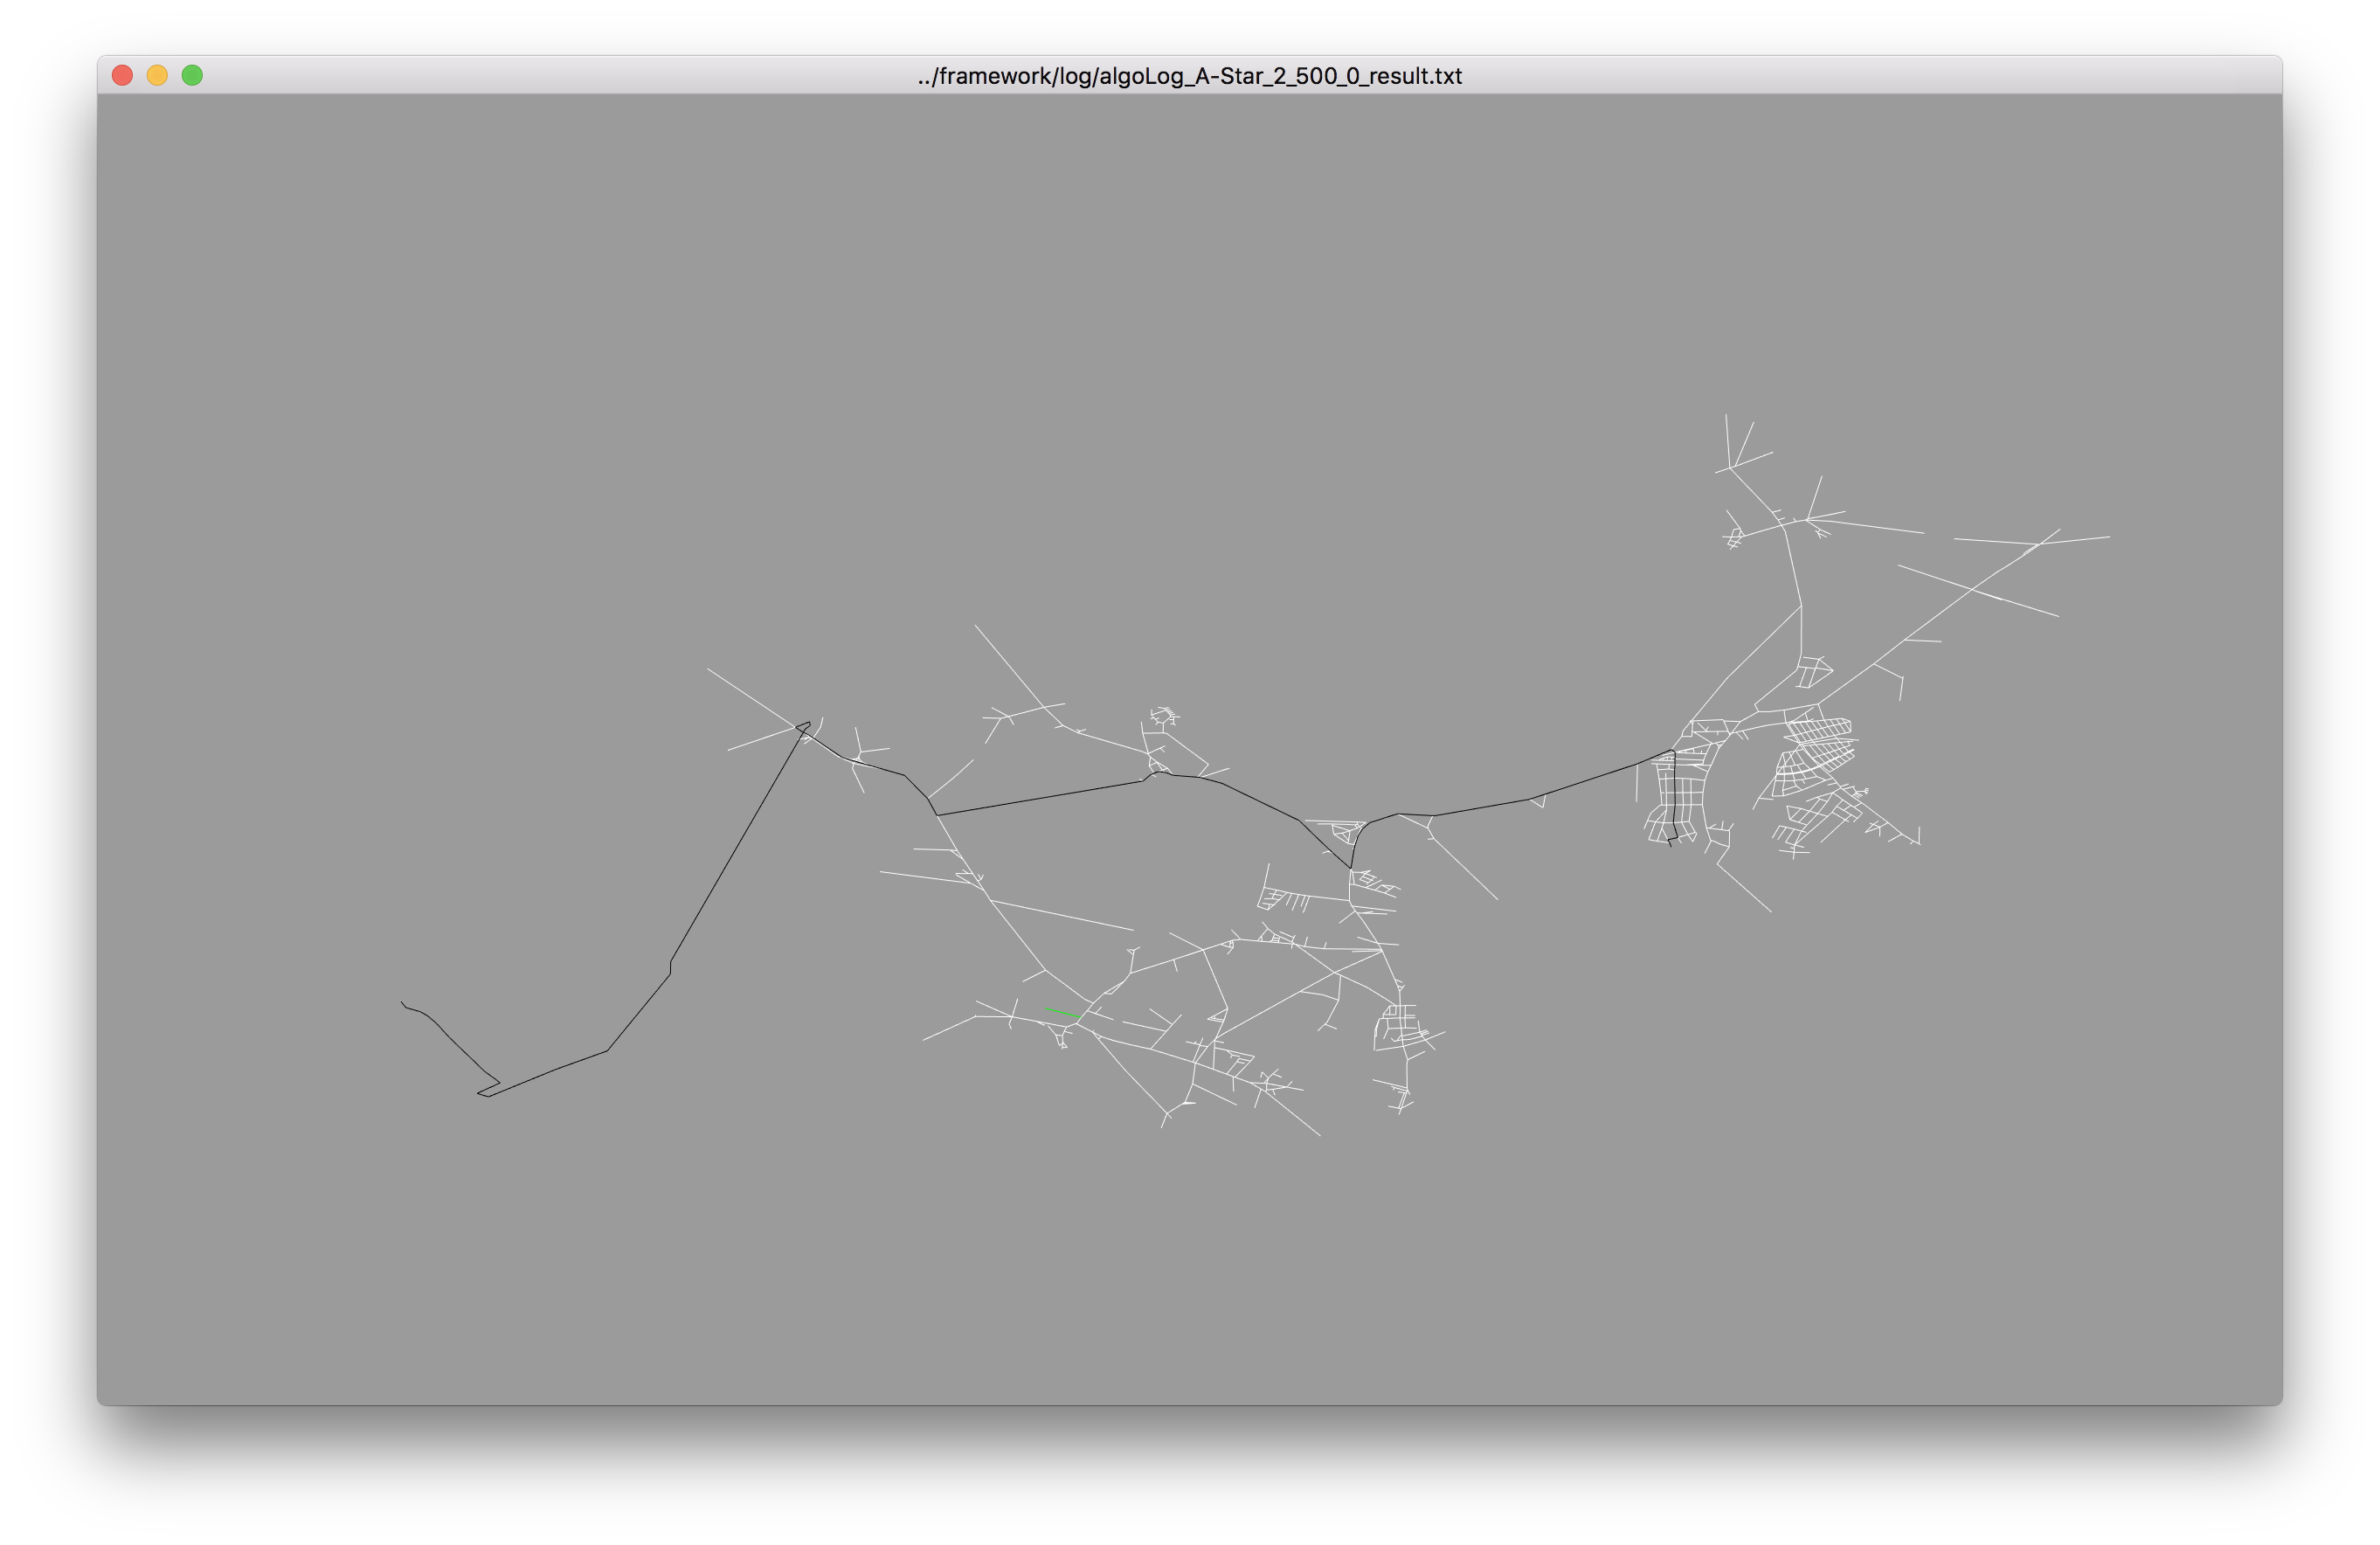
\includegraphics[width=0.5\textwidth]{Images/vis-edges-only-small.png}
	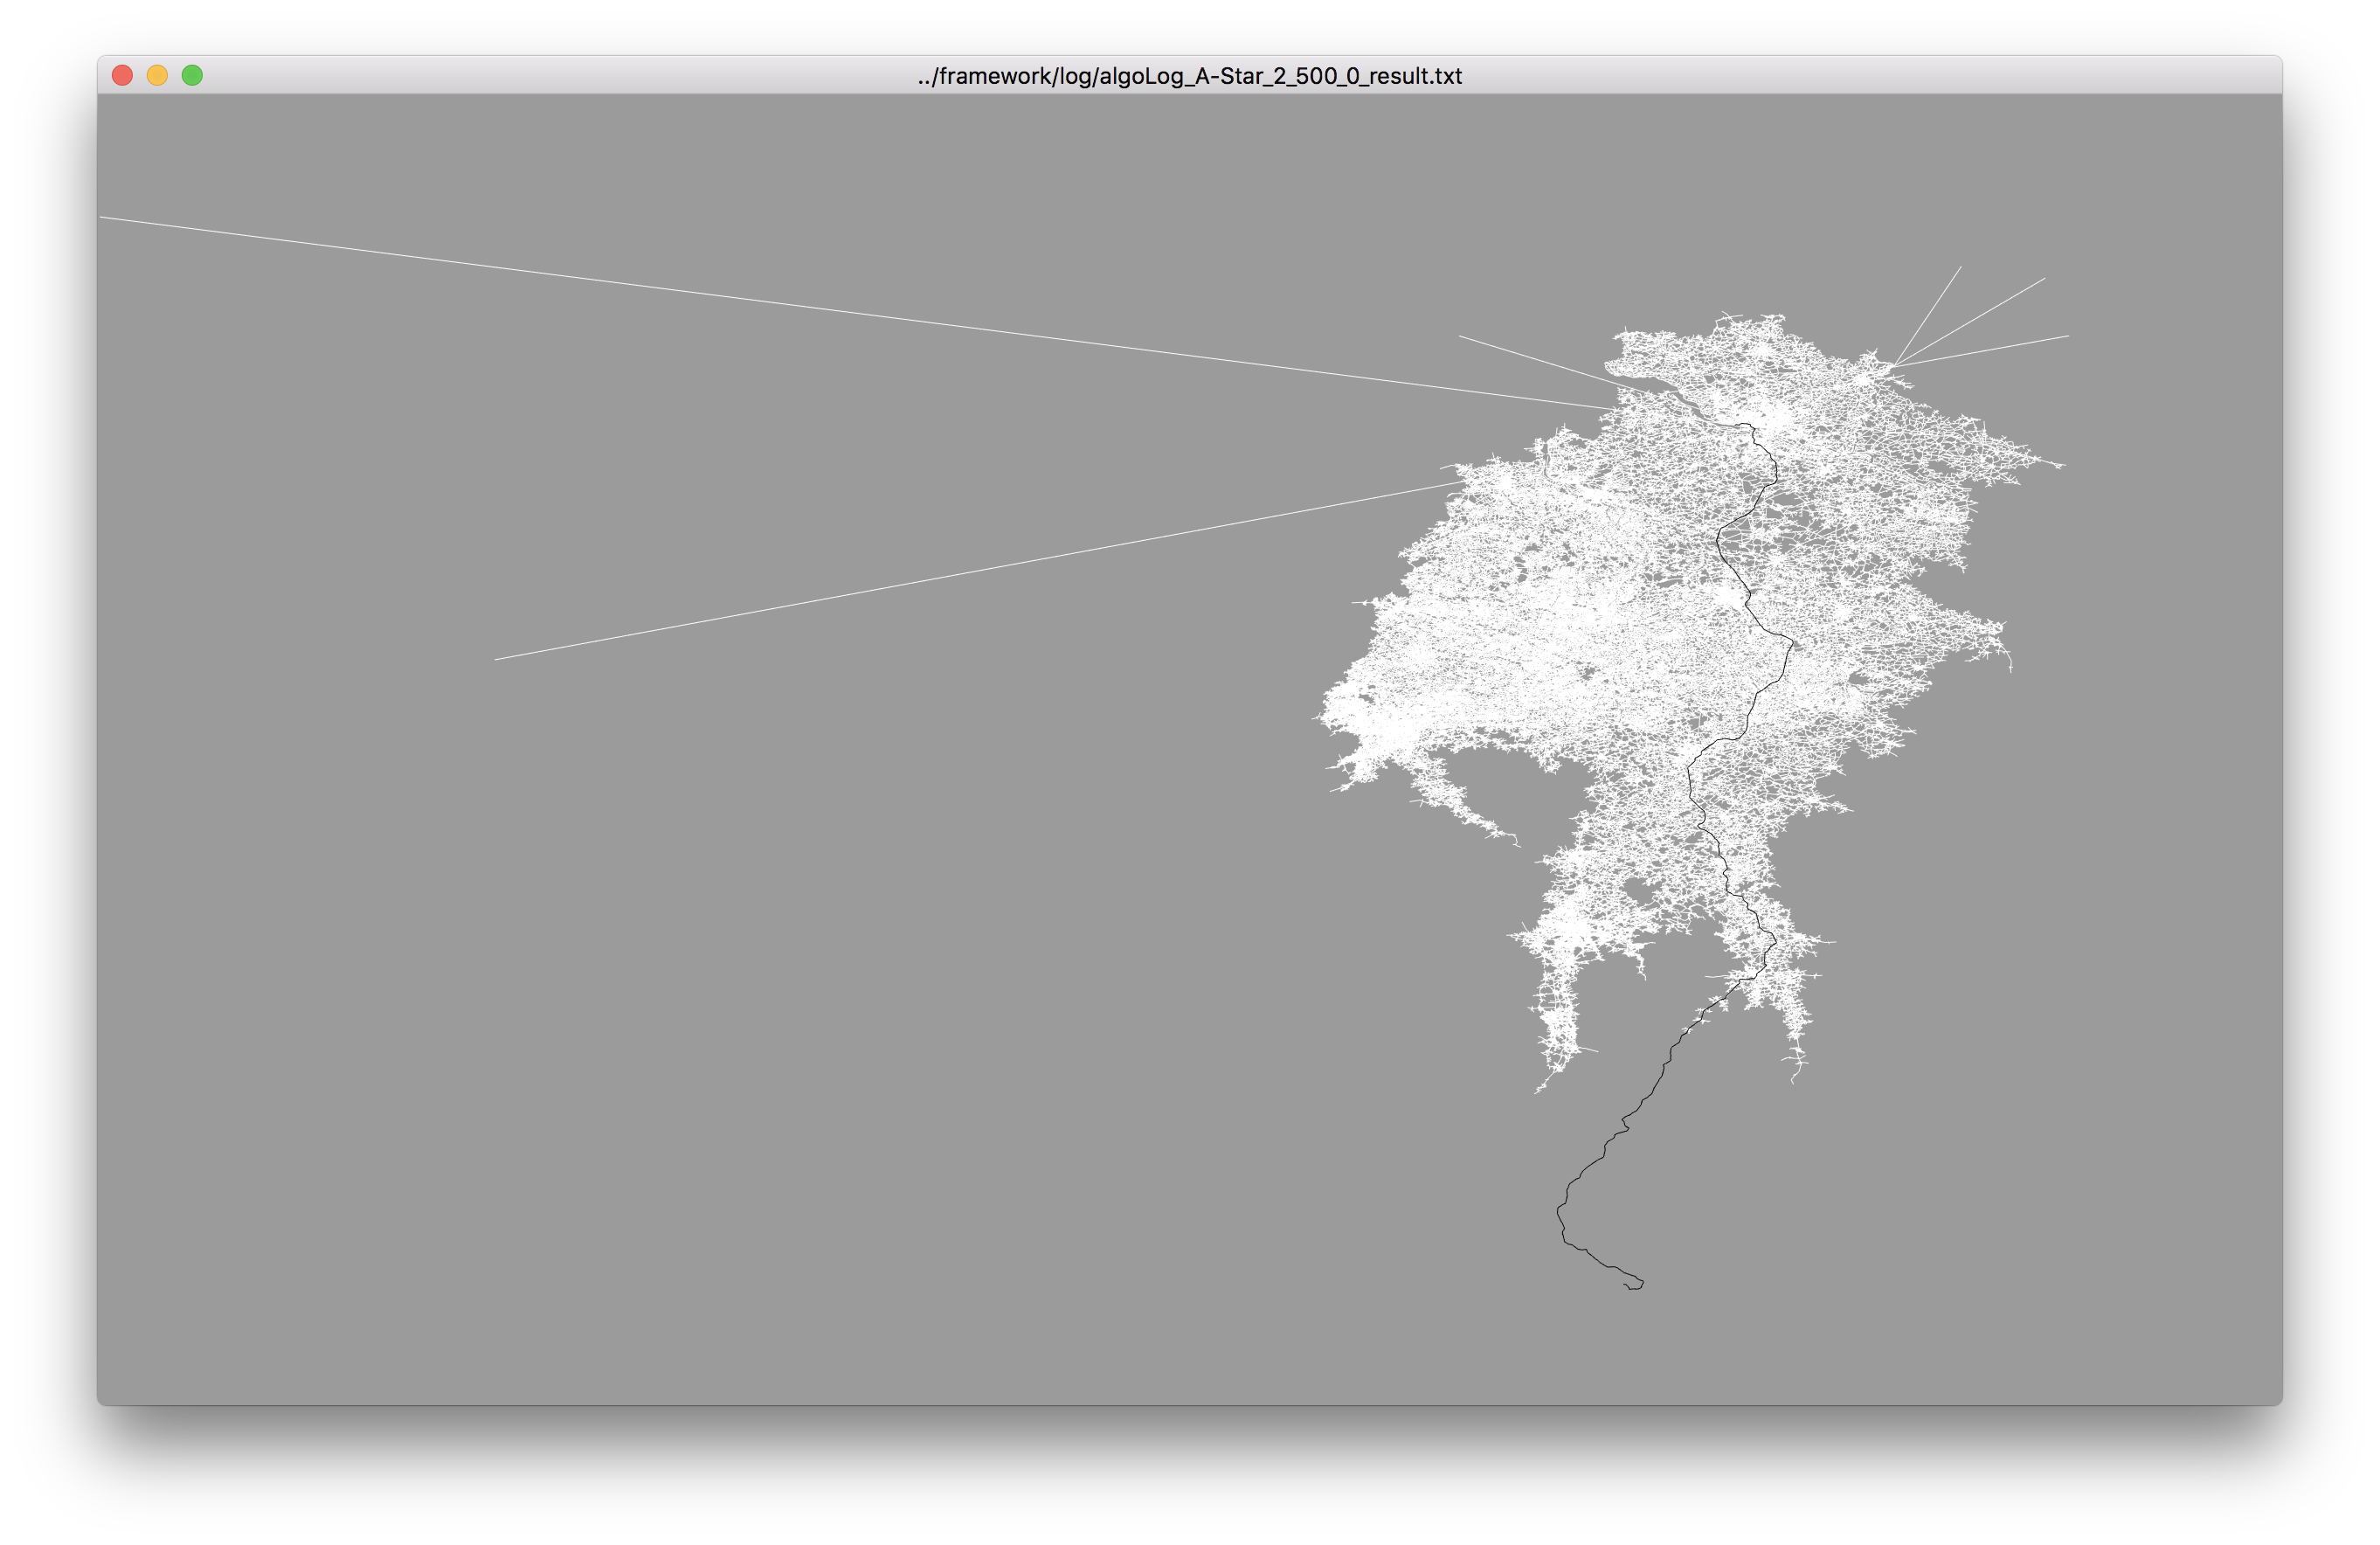
\includegraphics[width=0.5\textwidth]{Images/vis-edges-only-big.png}
\caption[]{Displaying all edges loaded}
\label{fig:basic_tiles}
\end{figure}


As a result we can see a basic tile structure in the visualization which leads to a basic understanding about the tiles loaded during the algorithm.
However as the algotithm evolves and the displayed graph grows tiles become much harder to distinguish from each other and especially in the inner graph it is not possible anymore to differentiate between different tiles.
Therefore we want to add a new type of elements to the visualization that will then represent the tiles.
As we use the Equirectangular projection, as mentioned in \cref{graph}, every tile is rectangular and has the same size.
Hence it is possilbe to add rectangulars around the tiles without any bigger effort.

\begin{figure}[H]
	\includegraphics[width=0.5\textwidth]{Images/placeholder.png}
\caption[]{Representing tiles through rectangles.}
\label{fig:rectangle_tiles}
\end{figure}


As visible in \cref{fig:rectangle_tiles} it is now possible to identify the single tiles clearly.
Furthermore the rectangles became the most important source of information on a higher level as we can recognize single edges only barely.
The biggest value added by the edges on this level is the information about the current step of the algorithm which is as the edges itself difficult to recognize.
As we want to change this, we will transfer this information to a higher level and therefore color the tile the algotihm is currently processing.
As a result we can now stop displaying the edges which makes the visualization much more uncluttered and leads to a major performance boost.

\begin{figure}[H]
	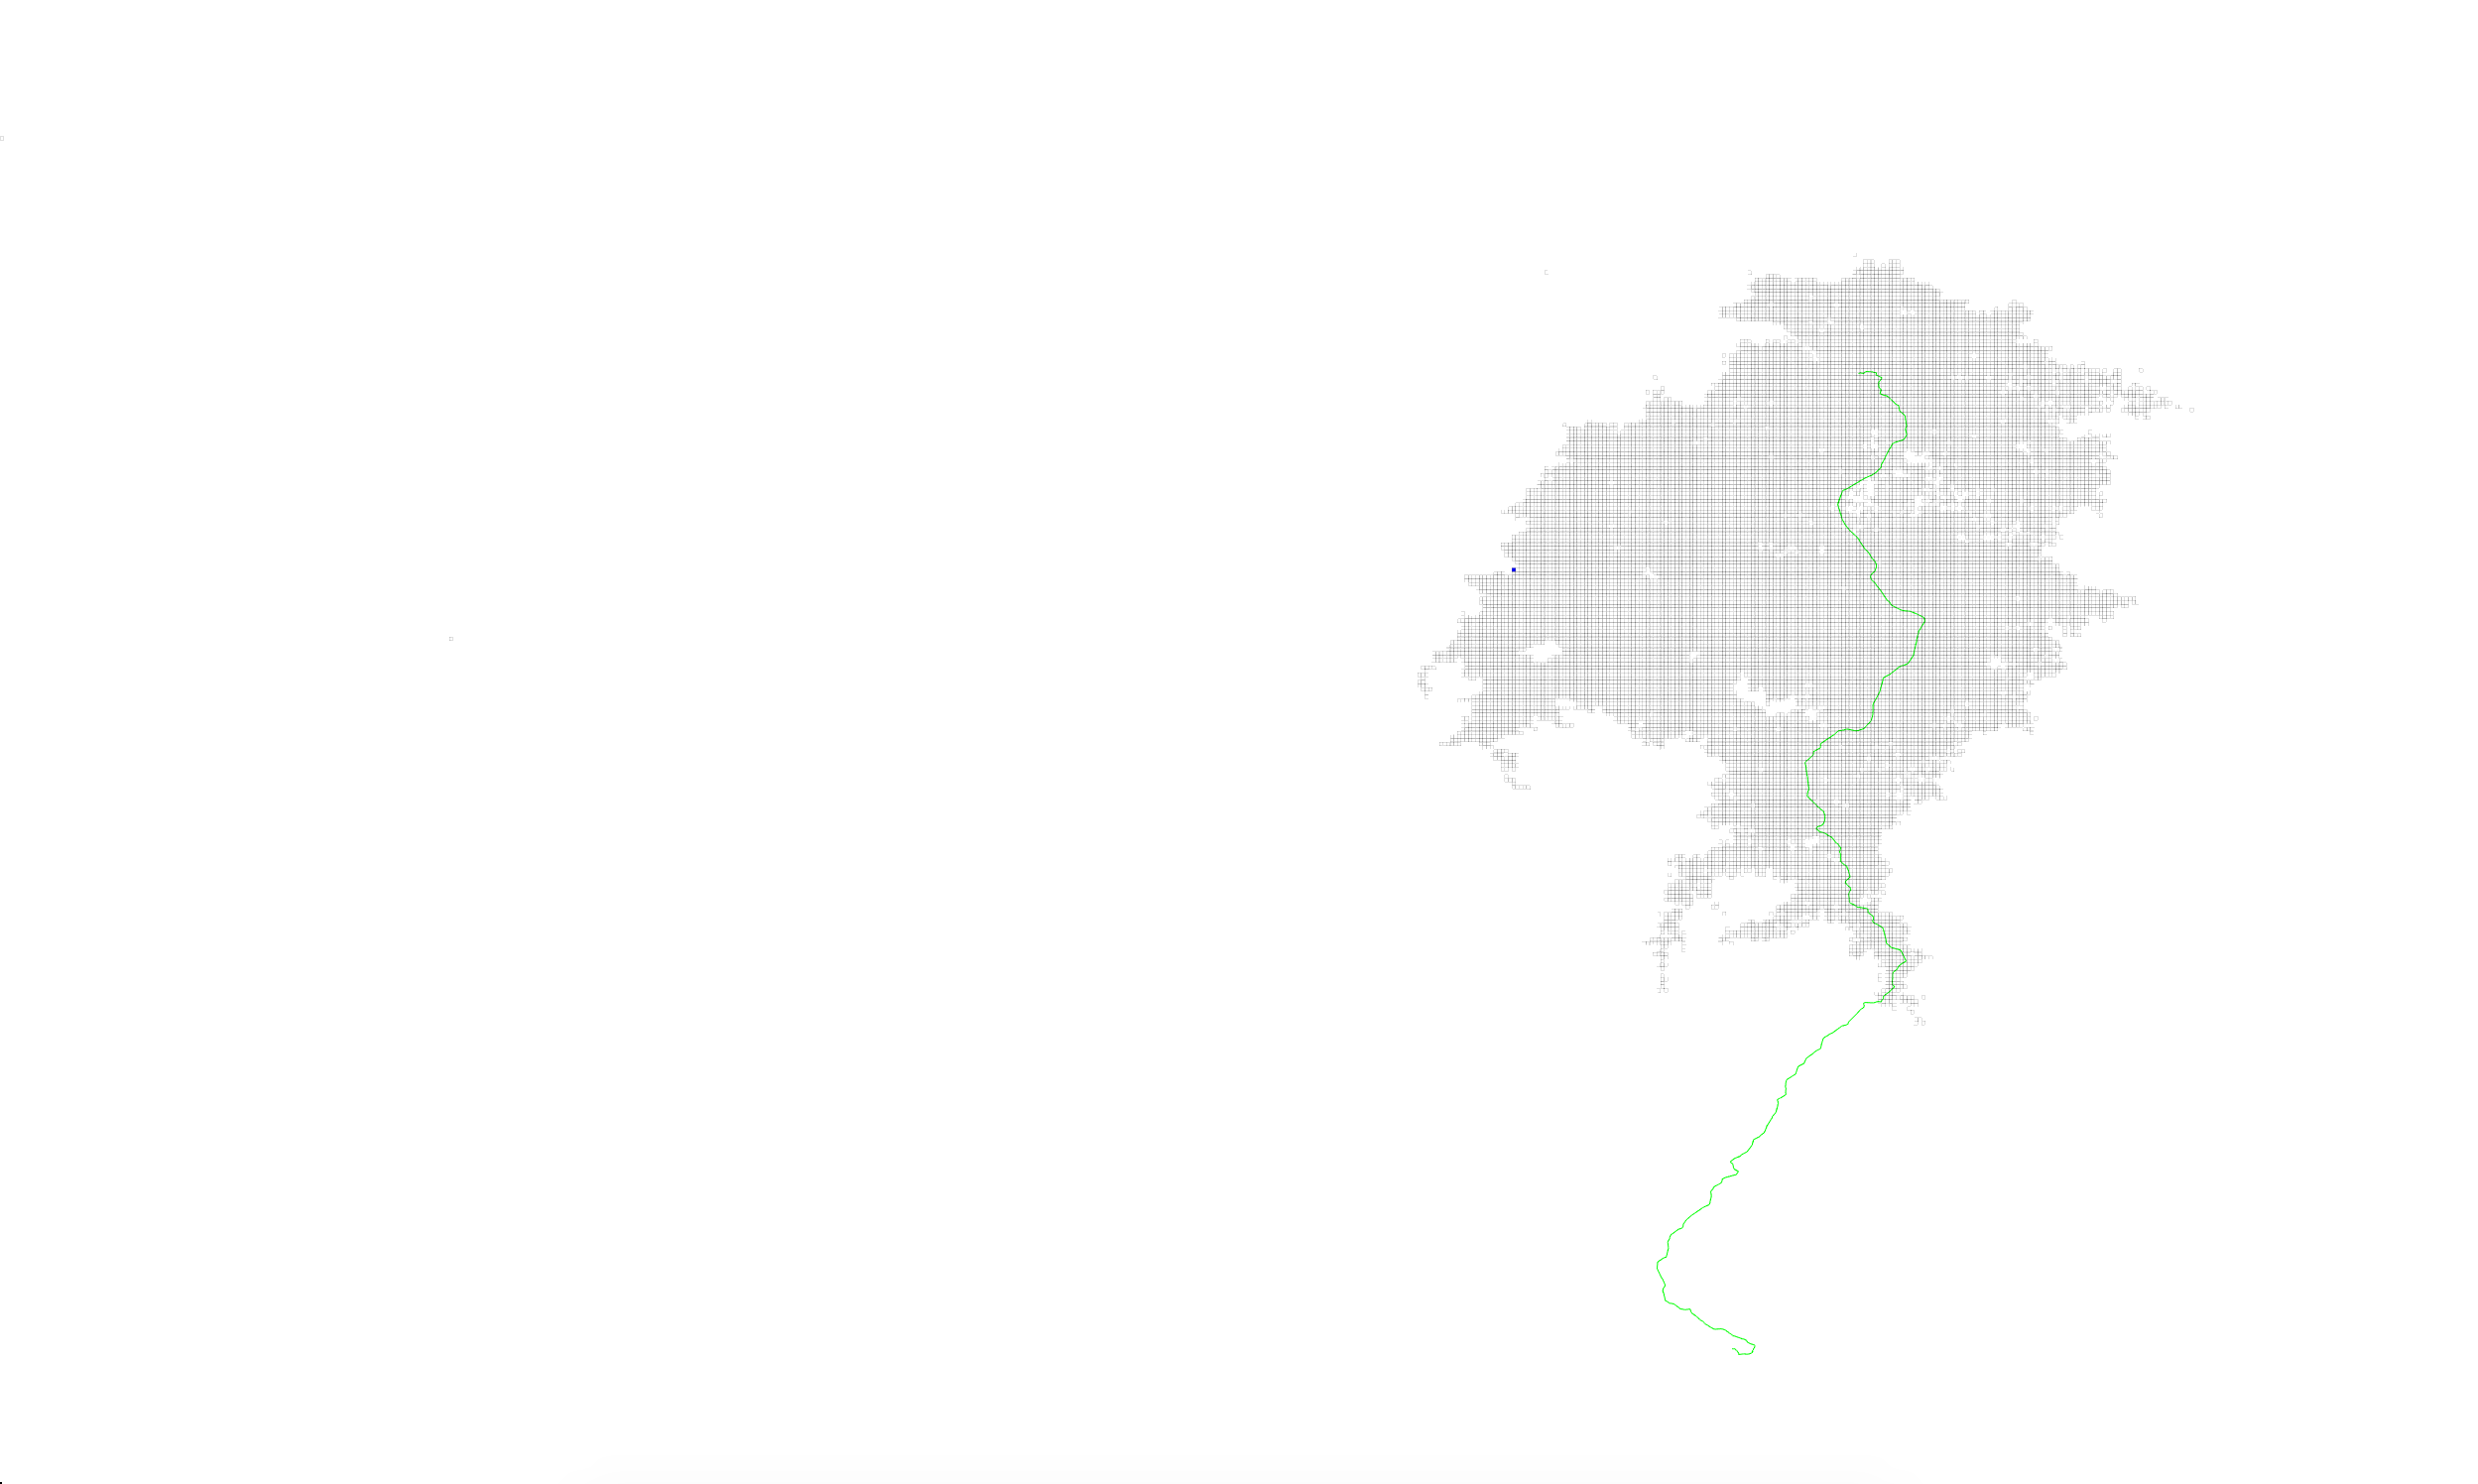
\includegraphics[width=\textwidth]{Images/vis-current-tile.png}
\caption[]{Representing tiles through rectangles.}
\label{fig:color_current_tile}
\end{figure}


In \cref{fig:color_current_tile} we see that we got a tile based visualization now.
Even though this visualization is still clean on a higher level, understanding the actuall approach of the algorithm is still hard, as the processed tile is colored to short to really process the information.
Hence we want to try to fix this by introducing aging of tiles.
This means that the currently processed tile is still collored but different than in the aproach befor it doesn't directly lose its color, but slowly.
In every step of the algorithm the tile is becoming a bit brighter.

\begin{figure}[H]
	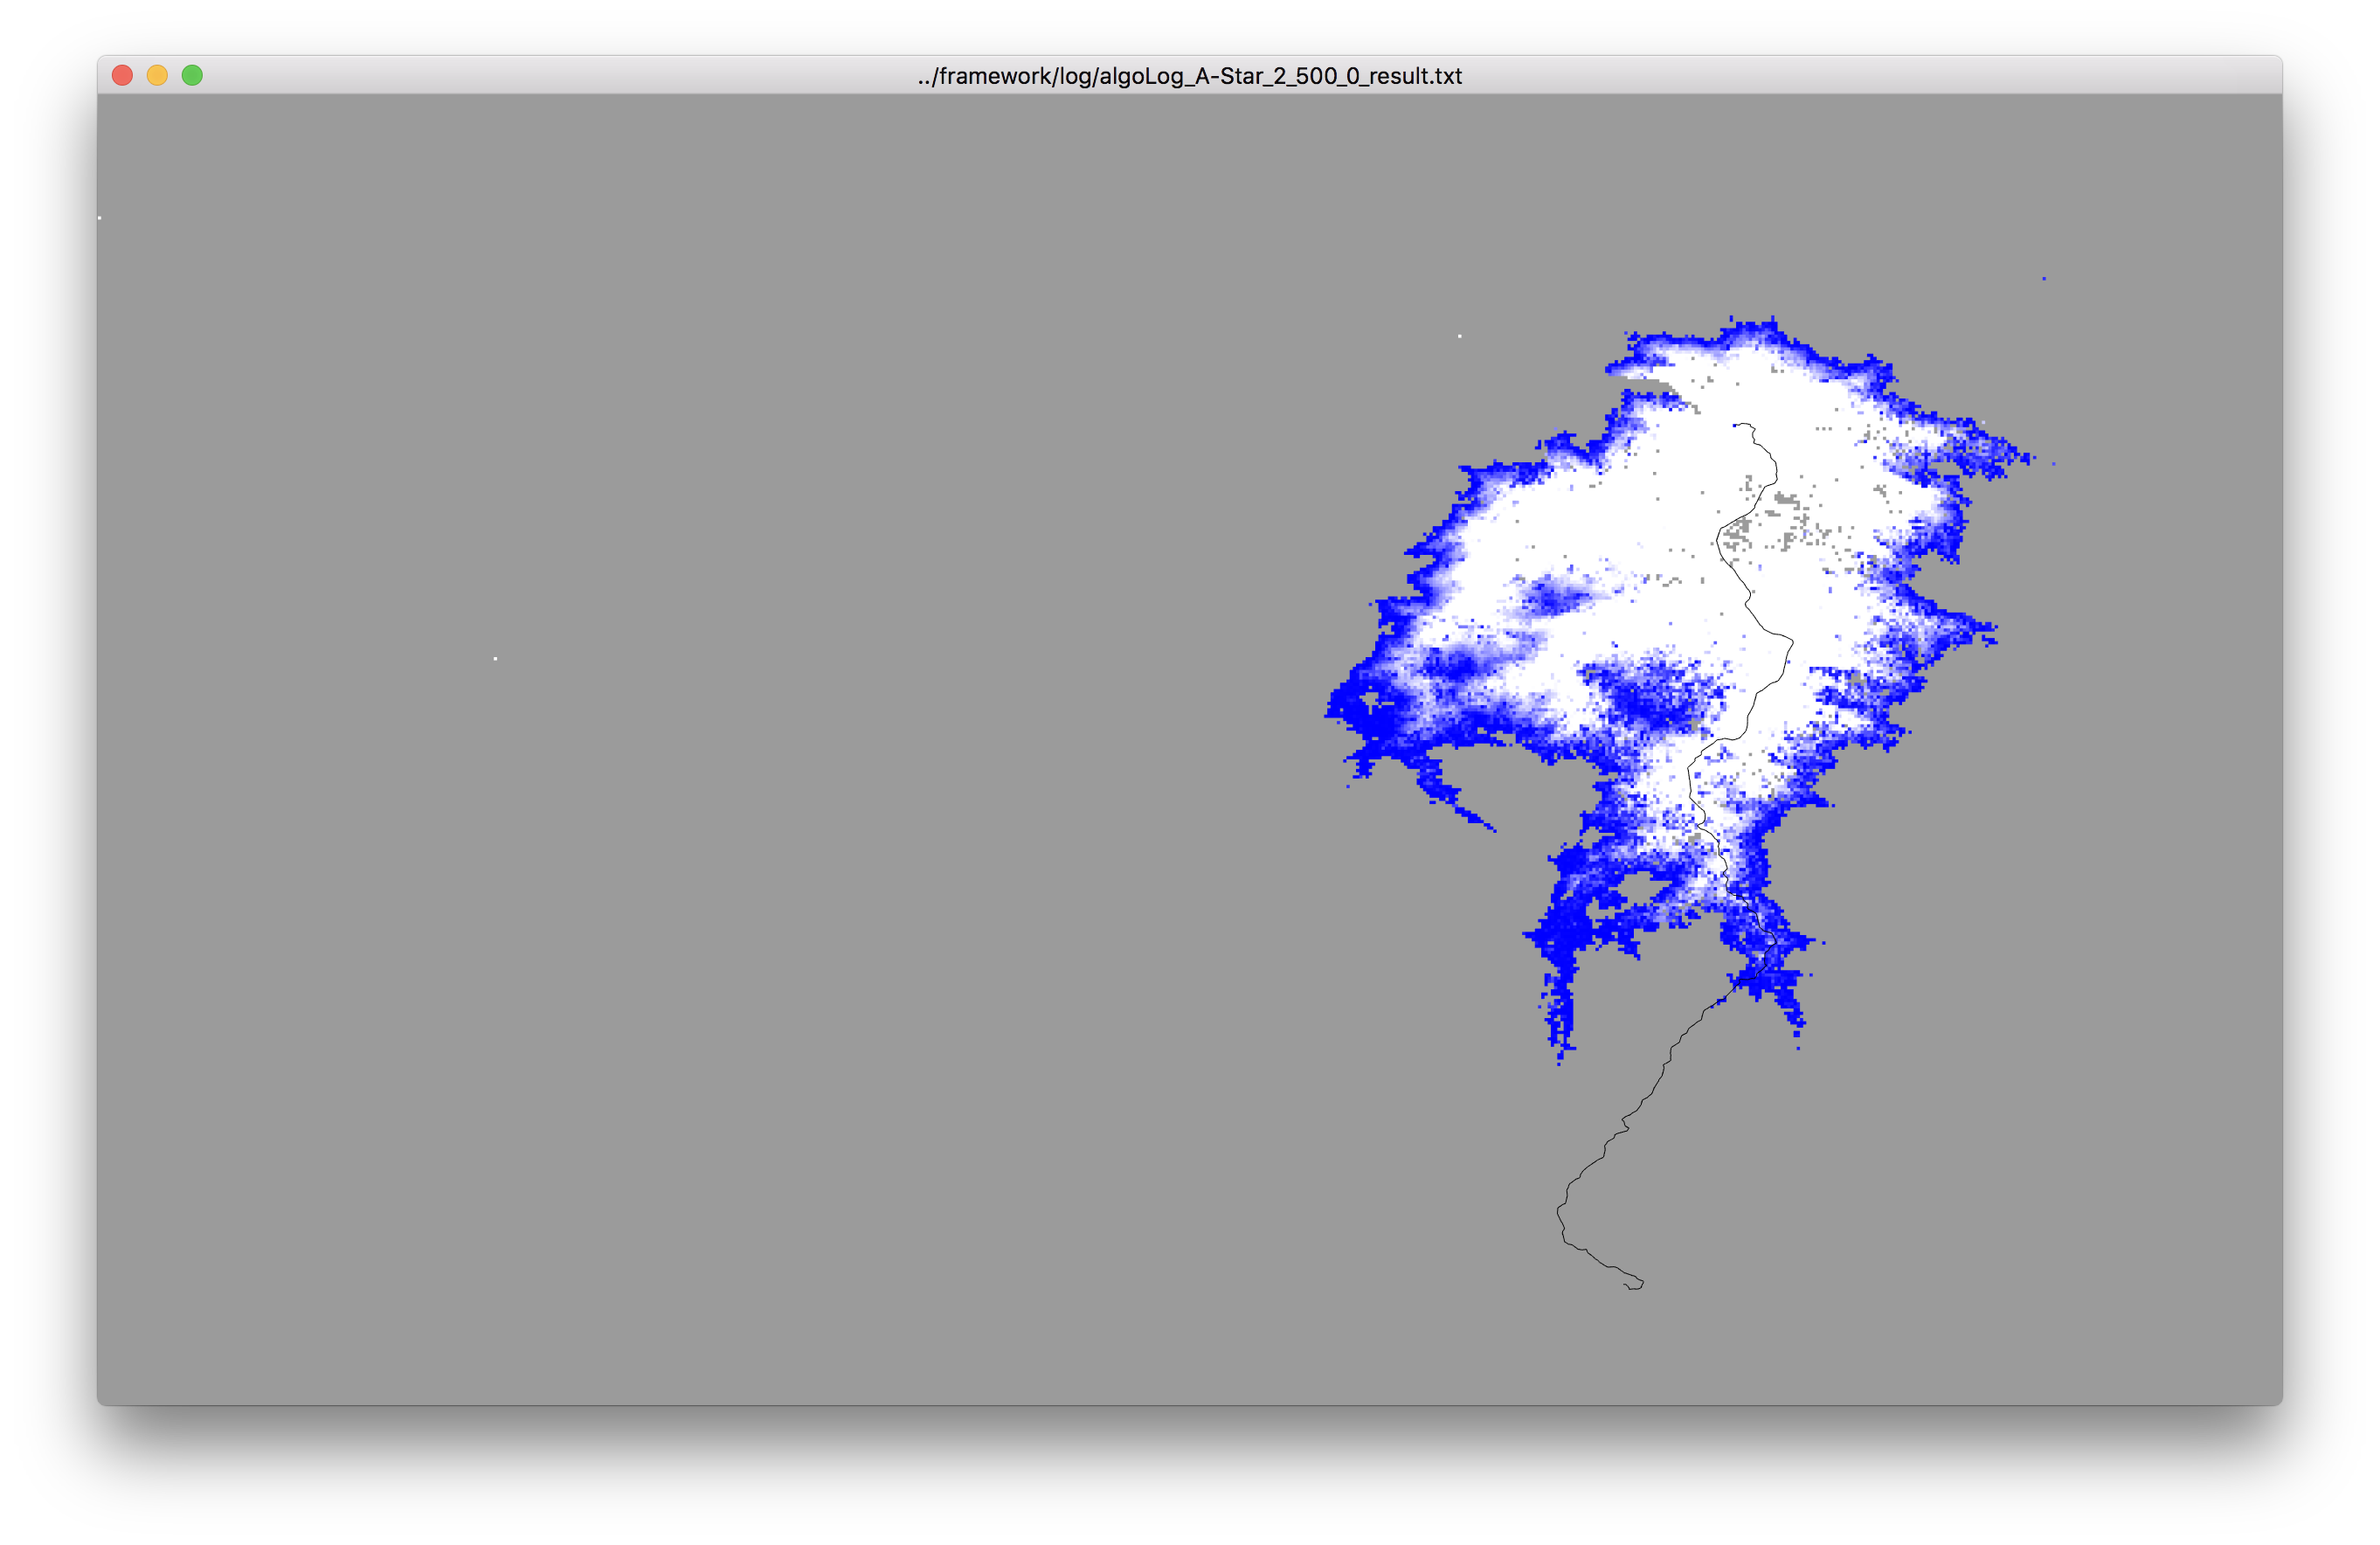
\includegraphics[width=\textwidth]{Images/vis-aged-coloring.png}
\caption[]{Displaying earlier loaded tiles darker.}
\label{fig:color_aged_tile}
\end{figure}


In \cref{fig:color_aged_tile} we see that this aproach strongly simplifies the way of acces information and leads to a much better understanding of the sequence of accesses.


\subsection{Visualizing the Cache}

In \cref{specification} explained that tiles are loaded in the cache, a fast storage
of limited size, before they are accessed.
Whenever a tile that is in the cache needs to be accessed by the algorithm no additional costs arise.
Therefore the loading of tiles into the cache the most expensive operation.
Scince the cache plays such a big role it should not be ignored during the visualization as well.
Because we already introduced the tiled visualization in \cref{tiles} we have a good foundation to work with.
As a first aproach we will color all the tiles that are currently stored in the cache and therefore directly accessible for the algortihm.



\begin{figure}[H]
	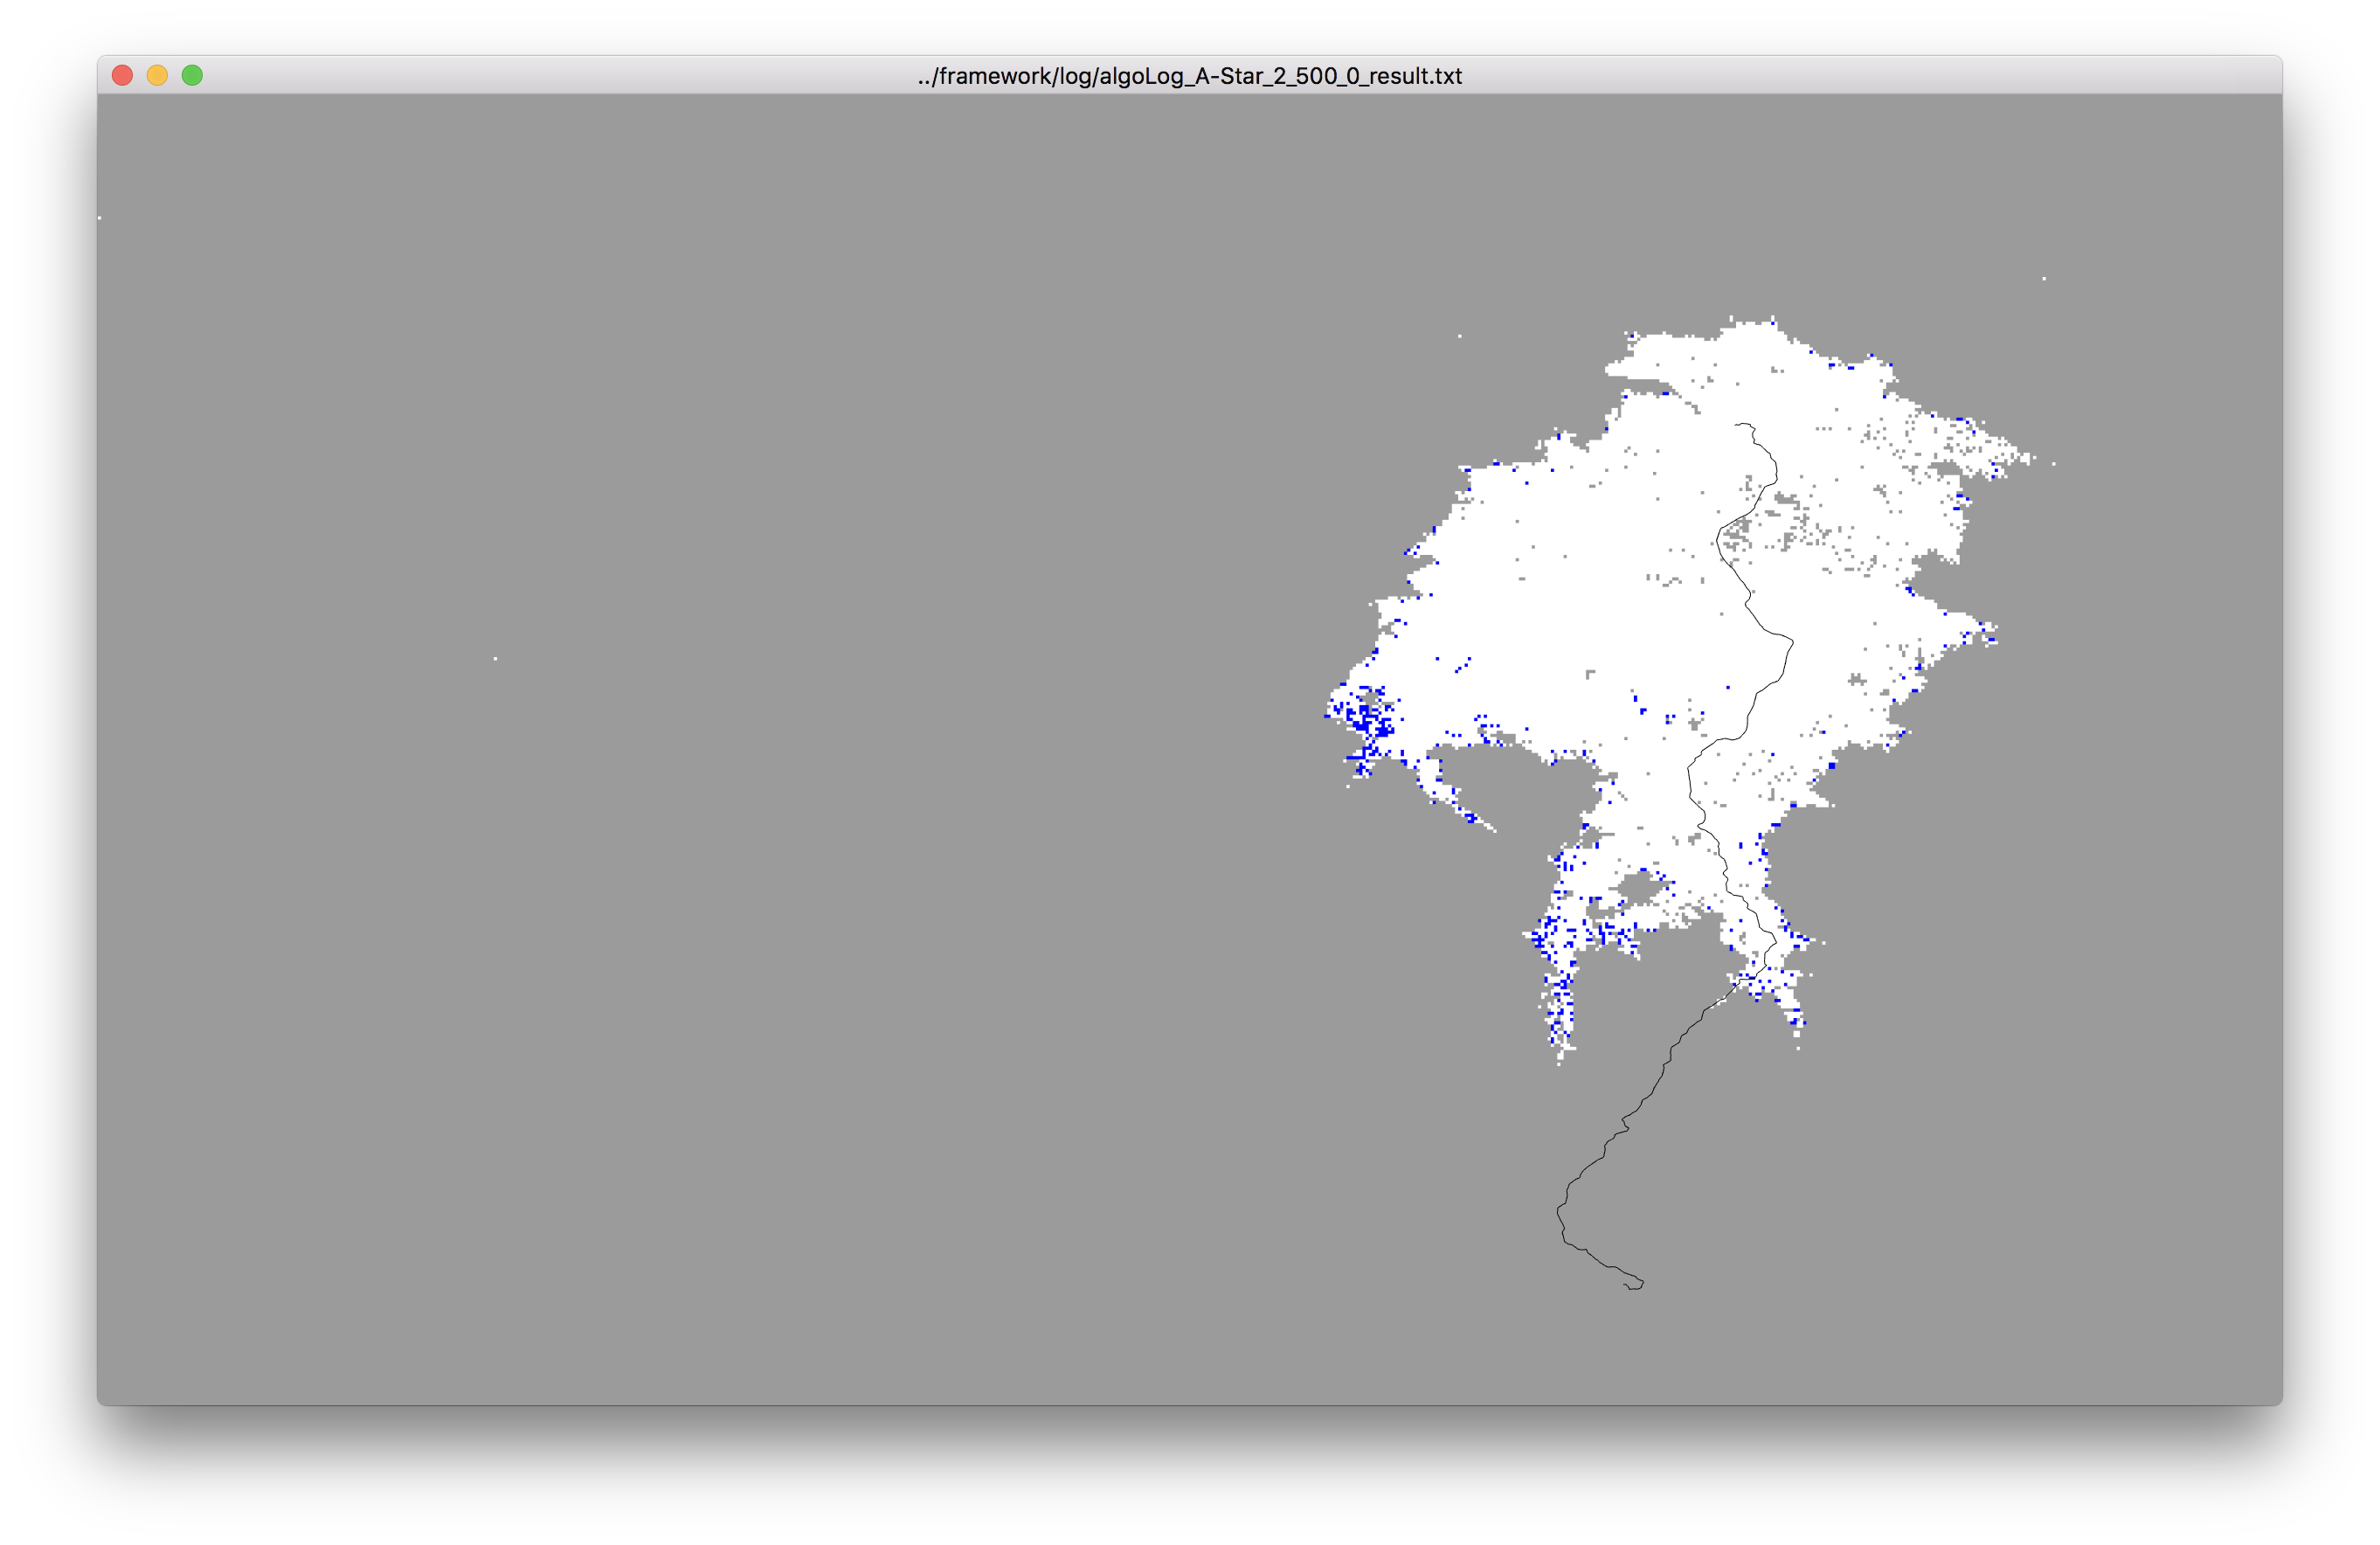
\includegraphics[width=\textwidth]{Images/vis-basic-cache.png}
\caption[]{Representing the cache by coloring tiles.}
\label{fig:cache_coloring}
\end{figure}


As we can see in \cref{fig:cache_coloring} the aged based coloring is not neccessary anymore. Due to the colored cache we archieved an improved understanding of past loaded tiles and the aged based coloring would futhermore distract from the important cache.

At this point it would be good to see how often a tile was loaded  in the cache, by only seeing one point of the visualization, without knowing what happened before.
Therefore we now want to color all the tiles except those who are in the cache according to the frequency they have been loaded.
Now a tile would be white after the initial loading and with every time it is loaded it would become a little redder.

\begin{figure}[H]
	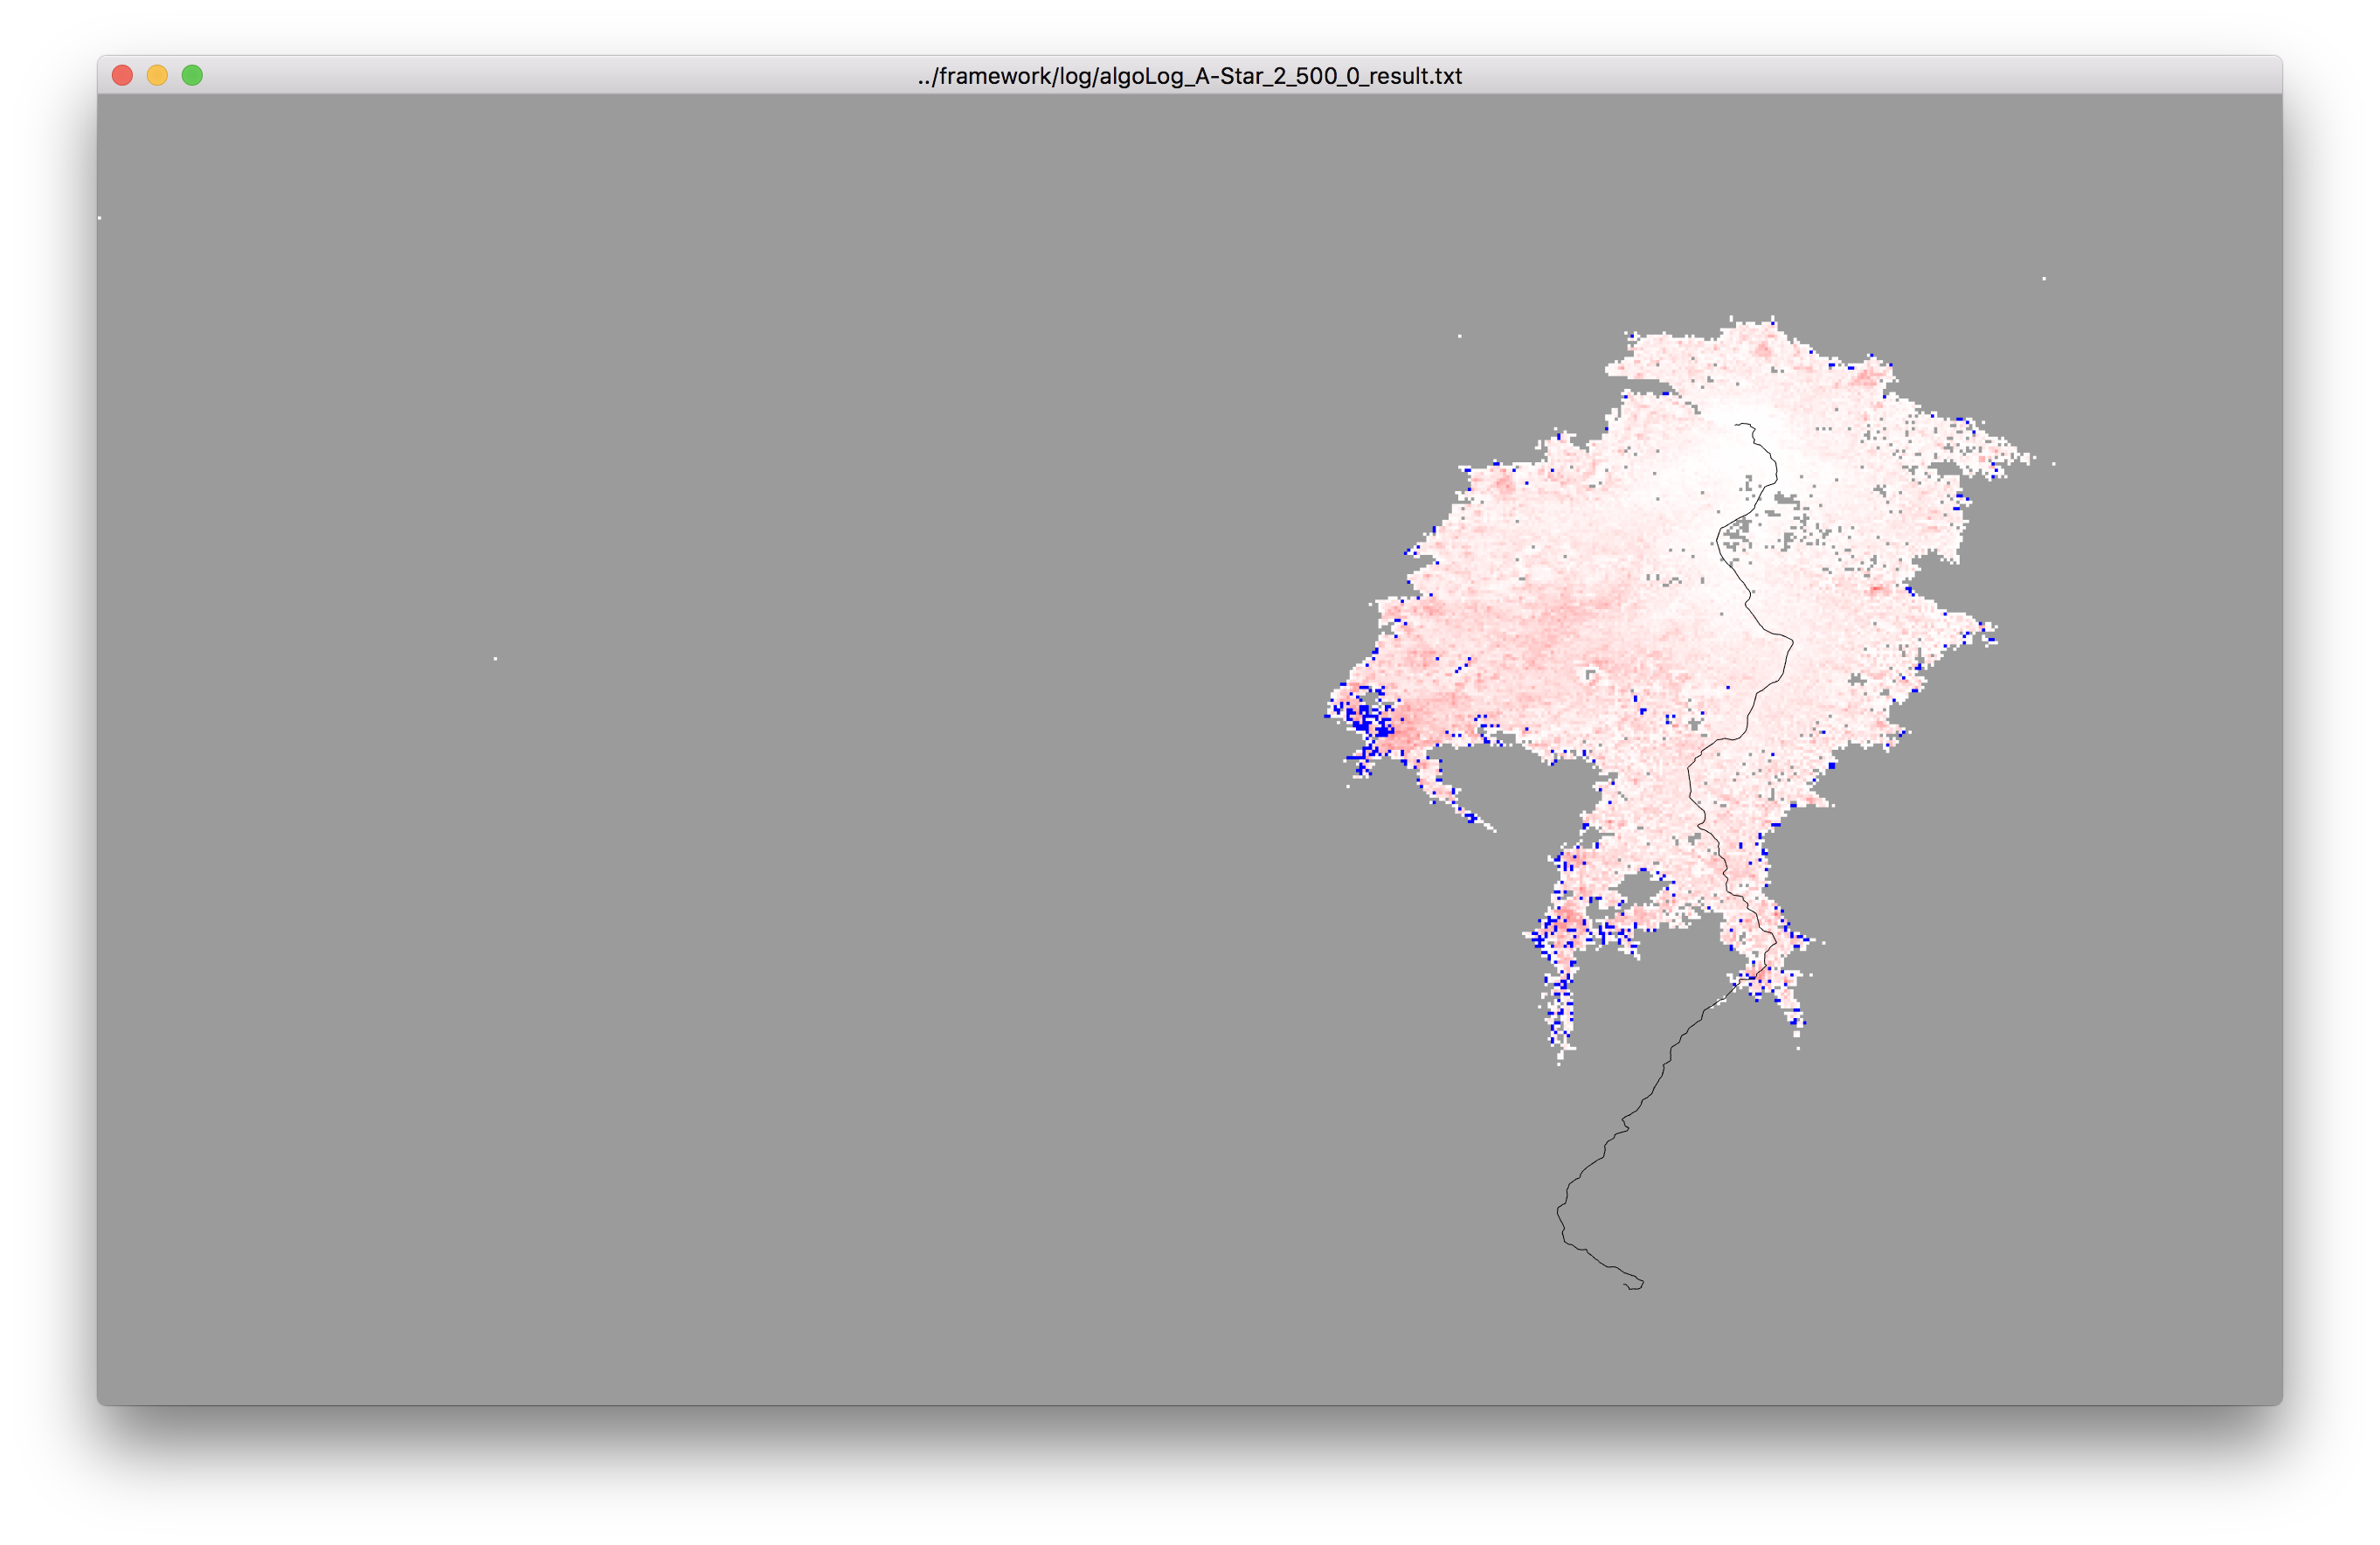
\includegraphics[width=\textwidth]{Images/vis-rgb-cache.png}
\caption[]{Coloring the tiles according to the amount of reloads.}
\label{fig:reload_coloring_white}
\end{figure}


By coloring the reloads this way, we can now see how good our algorithm performs and in which regions more reloading is happening.
Currently bigger reloadings are clearly visible, but when in comes to small differences those are only barely visible.
Therefore we want to try another color scale.
By setting the color of once loaded tiles to green and turn it into red the more the tile was loaded we hope to archieve a bigger and clearer contrast between slightly different tile loads.
\todo{discuss hsv?}

\begin{figure}[H]
	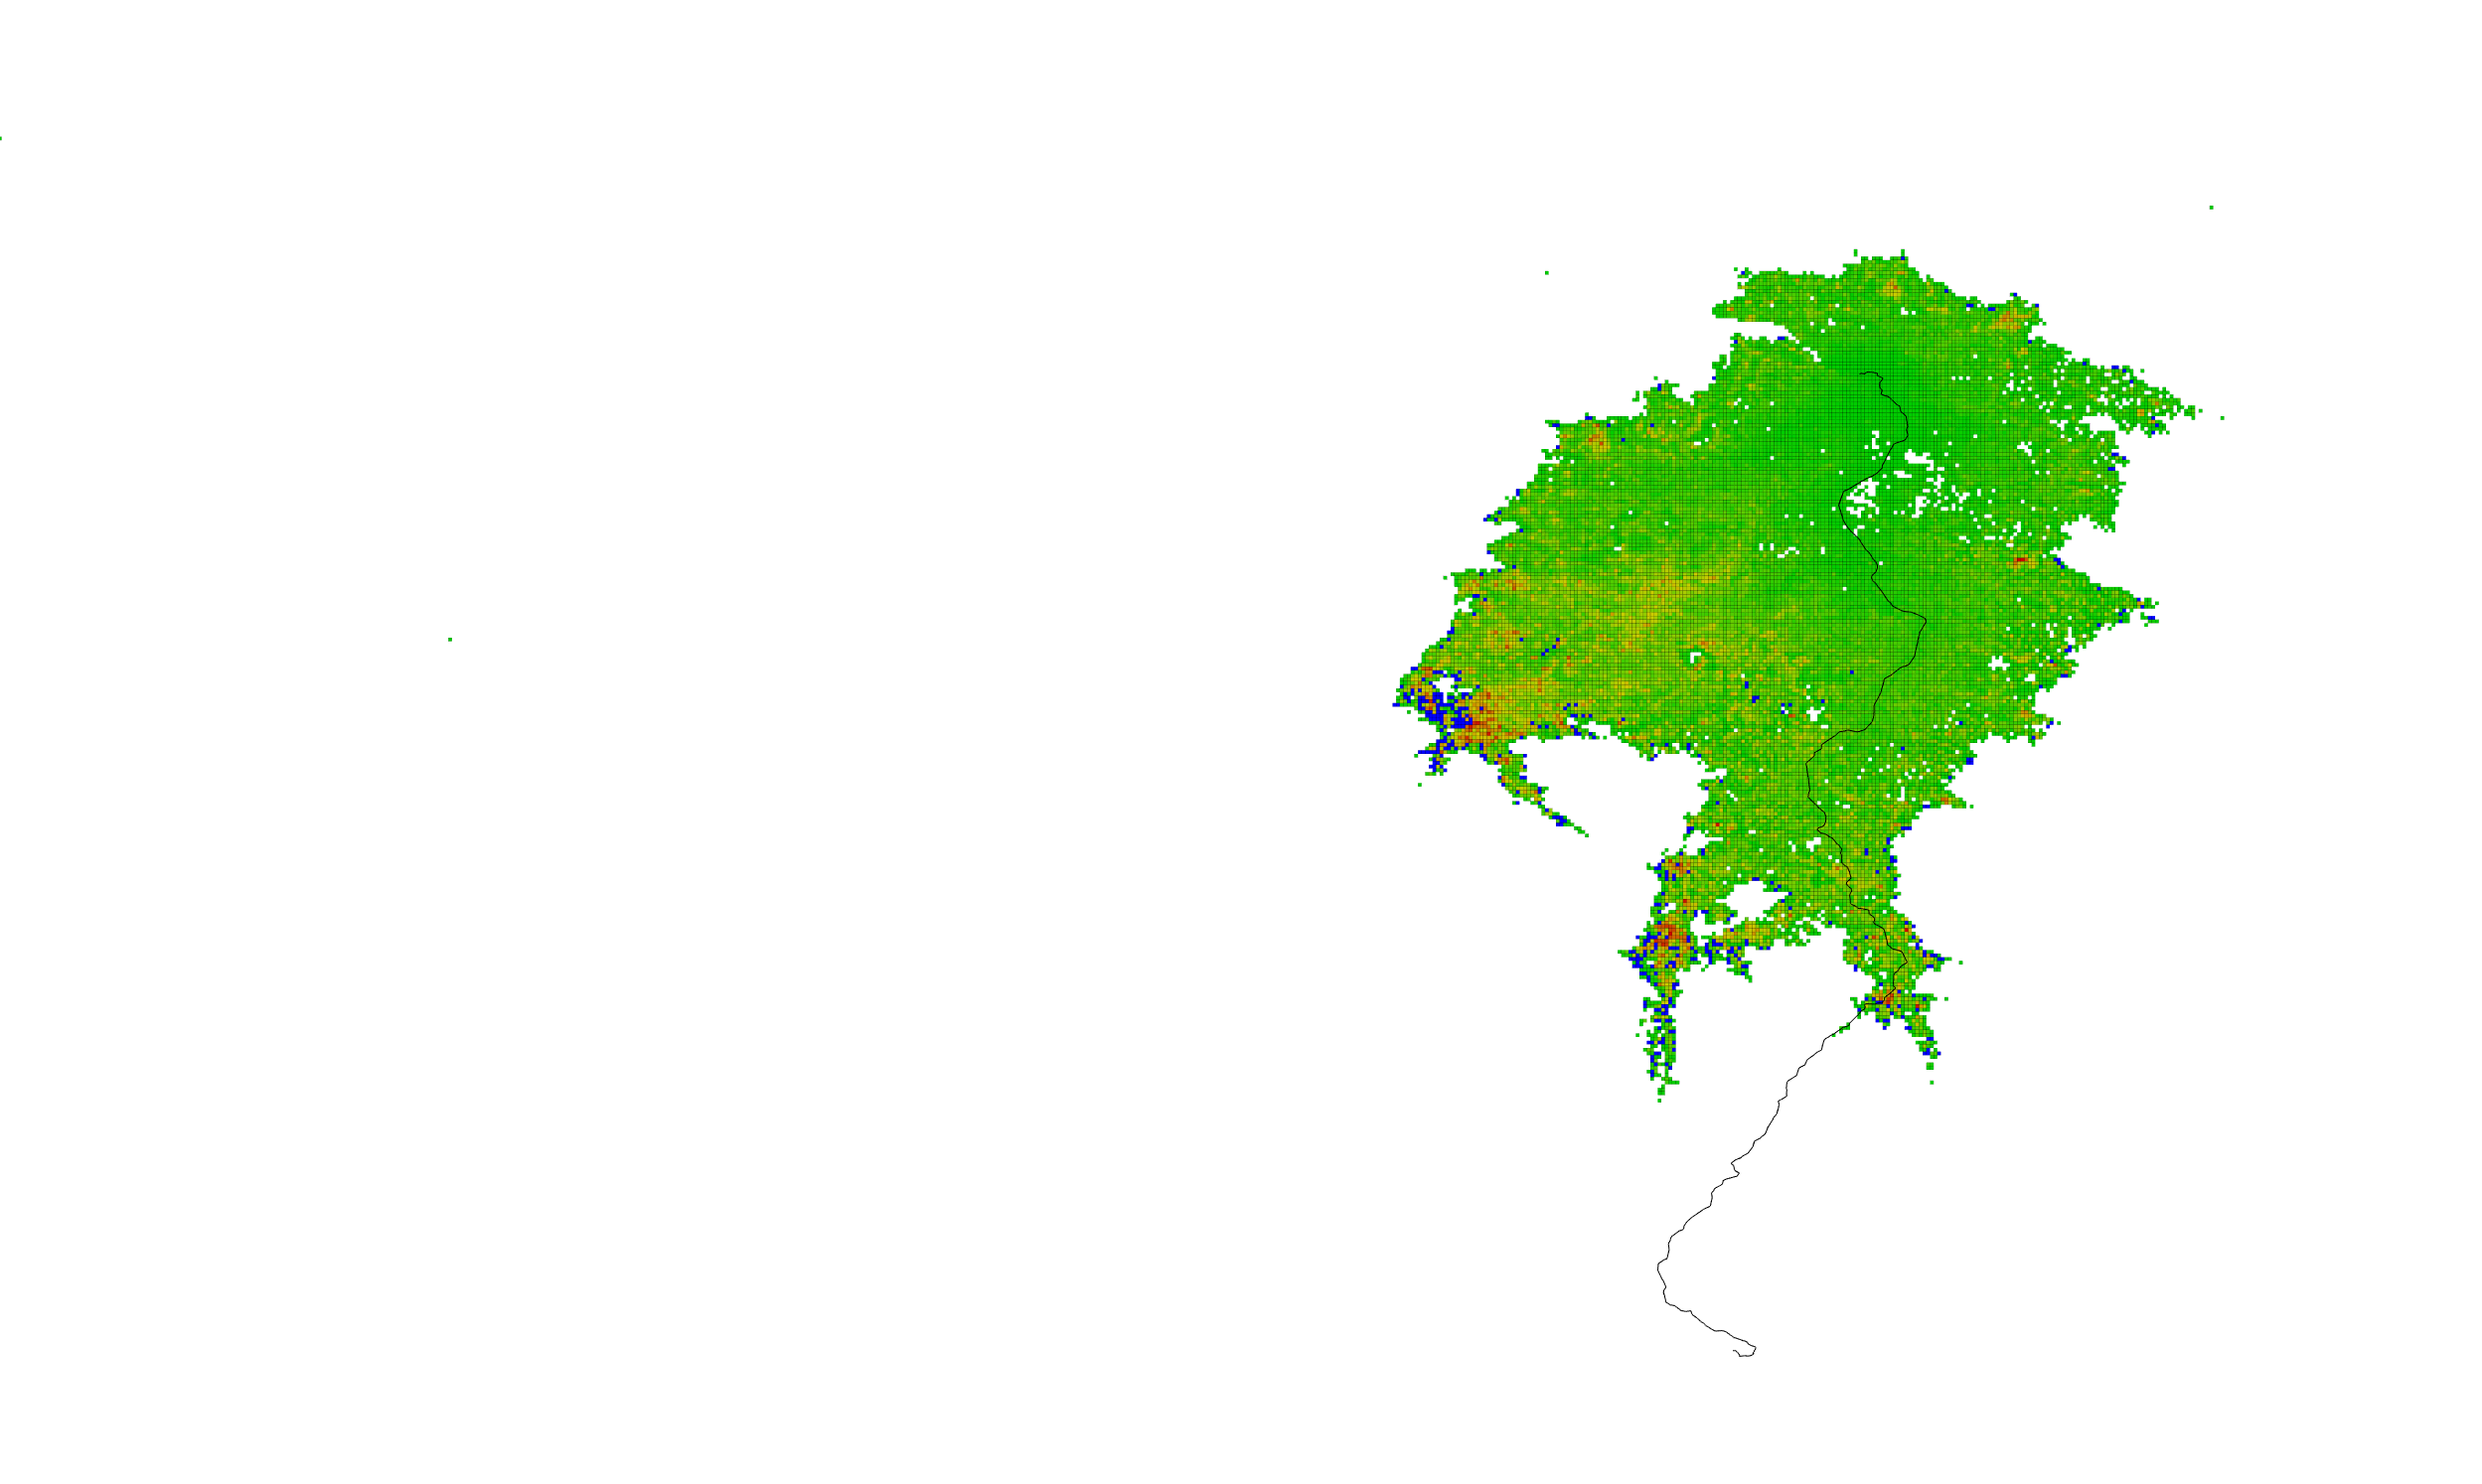
\includegraphics[width=\textwidth]{Images/vis-hsv-cache.png}
\caption[]{Changed color scheme. Now the tiles change their color from green to red.}
\label{fig:reload_coloring_white}
\end{figure}


As we see the different reload levels are now much easier to distinguish.


\section{Compare algorithms}

After having developed multiple algorithms comparing different algorithms becomes more important.
Therefore we could simply start two visualizations and display them next to each other.

\begin{figure}[H]
	\includegraphics[width=0.5\textwidth]{Images/placeholder.png}
\caption[]{Running two visualizations next to each other.}
\label{fig:two_visualization}
\end{figure}


As a result we would then see rough differences, for example in the search front, but smaller differences, as one a tile load more, are quite hard to see.
For comparing algorithms we therefore need  a new variation of our visualization.
The basic idea is to put two different algorithms over each other and so be able to compare two algortihms in one image.
Therefore we could just split each tile in two and color the left half according to the reloads of one algorithm and the right side according to the other.

\begin{figure}[H]
	\includegraphics[width=0.5\textwidth]{Images/placeholder.png}
\caption[]{Splittin the tiles.}
\label{fig:splitted tiles}
\end{figure}


We now have a much better way to compare two algorithms, as there is no distance anymore between the matching tiles but it is still difficult to clearly identify the differences without longer observation, as it is quite confusing.
For changing this we want to think about now if it really is  necessary to know how often a tile was loaded in a specific algorithm or if showing the difference between the tile-loads is enough.
For finding out, we will try out the second idea as well.
Therefore we calculate the difference between the amount of tile loads for each tile.
Then we display all the tiles that has been accessed by at least one algorithm and color those greenish that have been loaded more often by the first algorithm.Those which has been loaded more often by the second algotihm are colored reddish.
The more intense the color the bigger is the difference in the amount of tile loads.

\begin{figure}[H]
	\includegraphics[width=0.5\textwidth]{Images/placeholder.png}
\caption[]{Showing only the difference of tile loads.}
\label{fig:splitted tiles}
\end{figure}



\section{Miscellaneous}

In this section we will take a look on the visualization we have just build and think about some features that help to improve its accessibility.
As we are working on big graphs with thousands of nodes even the tiled vizualization might become quite small.
As we might want to look at a specific region more focussed we should be able to zoom into our navigation.
When zoomed in we also need to be able move our view to the region we want to look at.

\begin{figure}[H]
	\includegraphics[width=0.5\textwidth]{Images/placeholder.png}
	\includegraphics[width=0.5\textwidth]{Images/placeholder.png}
\caption[]{View on whole graph(left) vz Zoomed view(right)}
\label{fig:splitted tiles}
\end{figure}


An other idea to improve the information given by the visualization is to be able get some information about the edges.
This might be useful when we want to understand, why specific tiles are loaded much more then others.
On a high level view on the graoh this might not be usefull as the amount and the size of the edges would make it impossible to really get some information out of it, but as we are now able to zoom it becomes quite useful.

\begin{figure}[H]
	\includegraphics[width=0.5\textwidth]{Images/placeholder.png}
\caption[]{Viewing the graph itself in addition to the tiles.}
\label{fig:splitted tiles}
\end{figure}


This seems to be a good compromise between visualizing only the edges and visualizing only the tiles.
As we have some more information about the tiles we can also try to include them in the representation.
As the length of the edges is already represented by the length of the lines in the visualization we only got the speed left to put into the edges.
We will do this by coloring the edges according to their speed.
Starting with red for 0 Km/h and going up to red for up to 150 Km/h.

\begin{figure}[H]
	\includegraphics[width=0.5\textwidth]{Images/placeholder.png}
\caption[]{Speed based color sceeme.}
\label{fig:splitted tiles}
\end{figure}


\todo{Evaluate}

\chapter{Outlook}
\begin{itemize}
	\item verschiedene Projektionen
	\item knoten anordnen mit kanten mit länge = kosten
	\item different layers
	\item gerichtete edges
\end{itemize}



% \chapter{The Solutions}
%
% \section{Displaying Edges} \label{edges_only}
% As the nodes and edges seem to be the most important part of an algorithm the first approach of building our visualization was to draw all nodes and edges as soon as they were processed.
%
% \begin{figure}[H]
%     \centering
%     \includegraphics[width = 1.0\textwidth]{placeholder.png}
%     \caption[HPI logo]{\label{fig:edges_only}Edges-only visualization.}
% \end{figure}
%
% As we see the basic search front is shown in this visualization prette good, but every information about the tiles is missing.
% Therefore we start drawing every edge of a blocks as soon as they is accessed the first time.
%
% \begin{figure}[H]
%     \centering
%     \includegraphics[width = 1.0\textwidth]{placeholder.png}
%     \caption[HPI logo]{\label{fig:edges_only_blocks}Modification of the edges-only visualization. Unloaded edges in already loaded blocks are now plottet as gray lines.}
% \end{figure}
%
% As we see it is now possible to see the basic tile strucure the algorithm has to handle but there are still multiple shortcomes.
% When the algorithm watches already explored edges the user doesn't see any movement on the screen.
% Thus a big part of the algorithm stays unvisualized.
% In adition the tile structure is not recognizable on bigger graphs and particular in the inner graph.
%
% \section{Displaying tiles}
% As mentionioned in \cref{edges_only} the tile structure of the map is still not present enough in regard of their role for the algorithm.
% Hence we now want to represent the tiles by rectangles. As base we use the visualization from \cref{edges_only}.
%
% \begin{figure}[H]
%     \centering
%     \includegraphics[width = 1.0\textwidth]{placeholder.png}
%     \caption[HPI logo]{\label{fig:edges_only_blocks} Showing tile borders as soon as the first node was accessed. }
% \end{figure}
%
% By adding the rectangles to the visualization we solved the problem of unrecogniseable tile borders.
% But still there is big part missing in the visaulization-process. The problem of missing movement in the inner graph mentioned in \cref{edges_only} is still present.
% Hence we will take a look at possible solutions in the next sections.
% Since displaying all edges leads to a bad performance on a bigger routes and as they do not really add value to the visualization on a higher level we will continue using only the rectanglerepresentation of the tiles.
%
% \subsection{Time based coloring}
% The first aproach for solving this problem is to
%
% \subsection{Cache based coloring}
%
% \section{Displaying Graph in background}
%
% \section{Diff between Searchfronts}
%
% \section{basic features}
% - zoom\\
% - stepping threw time\\
%



% \chapter{Gedanken}
% NDS motivieren?
% Inwieweit das Projekt erklären?
% Einzelne Features:
% Wie genau auf Algorithmen eingehen?
% Nur verlinken?
% Erst Wünsche an Visualisierung?
%
% Historisch rangehen?\\
%
% Introduction\\
% Graphs important -> developing graph algorithms important -> Bad results/hard to imagine how the algorithm works in reality -> Visualizeing helps to access information -> Visualizing the algorithm -> bachelorproject -> problem -> building a visualization based on problem\\
% Main part\\
% historische rangehensweise? --> Motivation --> resultat --> relektieren --> repeat\\
% Fazit\\
% Resultat verallgemeinern --> Maß zwischen planen und baunen finden --> schnell beginnen --> feedback von nutzern\\
%
% Gliederung
% Einleitung
% Probleme
% 	Graphstruktur
% 	Wie stell ich den Graph dar?
% 		Wo ist welcher Knoten?
%
% 	Wie stelle ich den Algorithmus dar?
% 	Wie beziehe ich die Tiles ein?
% 	Wie stelle ich den Cache dar?
% Lösungen
% Ausblick und Fazit
%
% \chapter{Chapter}
%
% \lettrine[findent = -0.3 em, nindent = 0.7 em]{A}{} small example as proposed by~\citet{test}.\myfootnote[-0.2]{The footnote number shouldn’t be in superscript down here.} Just some text referring to~\Cref{fig:HPI} and citing~\citet{test2}.\myfootnote[-0.2]{And another footnote.}
%
% \begin{figure}
%     \centering
%     
\includegraphics[width = 9 cm]{HPI_Logo.pdf}
%     \caption[HPI logo]{\label{fig:HPI}That’s the logo of the HPI. Naturally, it comes without its obligatory safe zone.}
% \end{figure}
%
% \section{Section}
%
% \subsection{Subsection}
%
% \subsubsection{Subsubsection}
%
% \newpage
% More text.
% \newpage
% Even more text.

% References
\renewcommand*{\bibname}{References}
\bibliographystyle{abbrvnat}
\bibliography{Files/References}


\chapter*{Independence Declaration}
\addcontentsline{toc}{chapter}{Declaration of Authorship}
\thispagestyle{empty}

I hereby declare that the thesis submitted is my own unaided work. All direct or indirect sources used are acknowledged as references.\vspace{2 ex}

Potsdam, \today\\[6 ex]

\begin{flushleft}
    \begin{tabular}{p{5cm}}
        \hline
        \centering\footnotesize\printAuthor
    \end{tabular}
\end{flushleft}


\end{document}
